\section{The Ripley Data-Set}
The ripley data set\footnote{Pattern recognition and Neural Networks B.D. Riplely, Cambridge University press, \url{http://www.stats.ox.ac.uk/pub/PRNN/}} is a well know set used to test machine learning algorithms. The training and validation data are shown in figure~\ref{fig:ripleyVisual}. 
\begin{figure}
\centering
\tikzset{mark size=1}
\input{../src/tikz/ripleyTrainingWithAvg.tex}
\input{../src/tikz/ripleyWithAvg.tex}
\caption{Visualization of the binary classification ripley training and validation data set. The filled dots indicate the position of the average point for each set.}
\label{fig:ripleyVisual}
\end{figure}
A liner and radial basis function kernel will be used to classify the validation data set. Figure~\ref{fig:ripleyLinClass} shows the linear classifier on the training data set and the validation data based roc-curve. In this experiment it was observed that the linear classifier got 16.8\% or 42 of the 250 validation data points wrong. Due to the non-liner nature of the problem the radial basis function kernel was able to outperform its linear counterpart, only 2.4\% or 6 validation data points where incorrect. This perfomance difference is somewhat reflected in the roc curves shown on the right of figures~\ref{fig:ripleyLinClass}~~\ref{fig:ripleyClass}, the curve assosicated with the rbf-svm covers more area and has a lower standard-deviation. 

\begin{figure}
\centering
\tikzset{mark size=1}
\input{../src/tikz/ripleyLinClass.tex}
% This file was created by matlab2tikz.
% Minimal pgfplots version: 1.3
%
%The latest updates can be retrieved from
%  http://www.mathworks.com/matlabcentral/fileexchange/22022-matlab2tikz
%where you can also make suggestions and rate matlab2tikz.
%
\documentclass[tikz]{standalone}
\usepackage{pgfplots}
\usepackage{grffile}
\pgfplotsset{compat=newest}
\usetikzlibrary{plotmarks}
\usepackage{amsmath}

\begin{document}
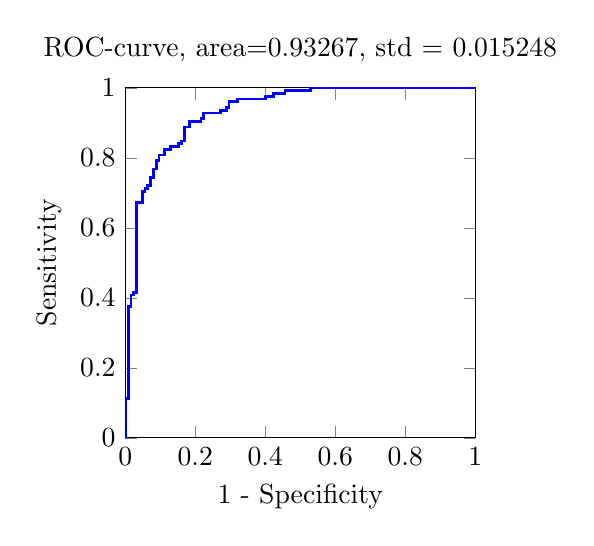
\begin{tikzpicture}

\begin{axis}[%
width=1.75in,
height=1.75in,
scale only axis,
xmin=0,
xmax=1,
xlabel={1 - Specificity},
ymin=0,
ymax=1,
ylabel={Sensitivity},
title={ROC-curve, area=0.93267, std = 0.015248}
]
\addplot [color=blue,solid,line width=1.0pt,forget plot]
  table[row sep=crcr]{%
0	0\\
0	0.008\\
0	0.016\\
0	0.024\\
0	0.032\\
0	0.04\\
0	0.048\\
0	0.056\\
0	0.064\\
0	0.072\\
0	0.08\\
0	0.088\\
0	0.096\\
0	0.104\\
0	0.112\\
0.008	0.112\\
0.008	0.12\\
0.008	0.128\\
0.008	0.136\\
0.008	0.144\\
0.008	0.152\\
0.008	0.16\\
0.008	0.168\\
0.008	0.176\\
0.008	0.184\\
0.008	0.192\\
0.008	0.2\\
0.008	0.208\\
0.008	0.216\\
0.008	0.224\\
0.008	0.232\\
0.008	0.24\\
0.008	0.248\\
0.008	0.256\\
0.008	0.264\\
0.008	0.272\\
0.008	0.28\\
0.008	0.288\\
0.008	0.296\\
0.008	0.304\\
0.008	0.312\\
0.008	0.32\\
0.008	0.328\\
0.008	0.336\\
0.008	0.344\\
0.008	0.352\\
0.008	0.36\\
0.008	0.368\\
0.008	0.376\\
0.016	0.376\\
0.016	0.384\\
0.016	0.392\\
0.016	0.4\\
0.016	0.408\\
0.024	0.408\\
0.024	0.416\\
0.032	0.416\\
0.032	0.424\\
0.032	0.432\\
0.032	0.44\\
0.032	0.448\\
0.032	0.456\\
0.032	0.464\\
0.032	0.472\\
0.032	0.48\\
0.032	0.488\\
0.032	0.496\\
0.032	0.504\\
0.032	0.512\\
0.032	0.52\\
0.032	0.528\\
0.032	0.536\\
0.032	0.544\\
0.032	0.552\\
0.032	0.56\\
0.032	0.568\\
0.032	0.576\\
0.032	0.584\\
0.032	0.592\\
0.032	0.6\\
0.032	0.608\\
0.032	0.616\\
0.032	0.624\\
0.032	0.632\\
0.032	0.64\\
0.032	0.648\\
0.032	0.656\\
0.032	0.664\\
0.032	0.672\\
0.04	0.672\\
0.048	0.672\\
0.048	0.68\\
0.048	0.688\\
0.048	0.696\\
0.048	0.704\\
0.056	0.704\\
0.056	0.712\\
0.064	0.712\\
0.064	0.72\\
0.072	0.72\\
0.072	0.728\\
0.072	0.736\\
0.072	0.744\\
0.08	0.744\\
0.08	0.752\\
0.08	0.76\\
0.08	0.768\\
0.088	0.768\\
0.088	0.776\\
0.088	0.784\\
0.088	0.792\\
0.096	0.792\\
0.096	0.8\\
0.096	0.808\\
0.104	0.808\\
0.112	0.808\\
0.112	0.816\\
0.112	0.824\\
0.12	0.824\\
0.128	0.824\\
0.128	0.832\\
0.136	0.832\\
0.144	0.832\\
0.152	0.832\\
0.152	0.84\\
0.16	0.84\\
0.16	0.848\\
0.168	0.848\\
0.168	0.856\\
0.168	0.864\\
0.168	0.872\\
0.168	0.88\\
0.168	0.888\\
0.176	0.888\\
0.184	0.888\\
0.184	0.896\\
0.184	0.904\\
0.192	0.904\\
0.2	0.904\\
0.208	0.904\\
0.216	0.904\\
0.216	0.912\\
0.224	0.912\\
0.224	0.92\\
0.224	0.928\\
0.232	0.928\\
0.24	0.928\\
0.248	0.928\\
0.256	0.928\\
0.264	0.928\\
0.272	0.928\\
0.272	0.936\\
0.28	0.936\\
0.288	0.936\\
0.288	0.944\\
0.296	0.944\\
0.296	0.952\\
0.296	0.96\\
0.304	0.96\\
0.312	0.96\\
0.32	0.96\\
0.32	0.968\\
0.328	0.968\\
0.336	0.968\\
0.344	0.968\\
0.352	0.968\\
0.36	0.968\\
0.368	0.968\\
0.376	0.968\\
0.384	0.968\\
0.392	0.968\\
0.4	0.968\\
0.4	0.976\\
0.408	0.976\\
0.416	0.976\\
0.424	0.976\\
0.424	0.984\\
0.432	0.984\\
0.44	0.984\\
0.448	0.984\\
0.456	0.984\\
0.456	0.992\\
0.464	0.992\\
0.472	0.992\\
0.48	0.992\\
0.488	0.992\\
0.496	0.992\\
0.504	0.992\\
0.512	0.992\\
0.52	0.992\\
0.528	0.992\\
0.528	1\\
0.536	1\\
0.544	1\\
0.552	1\\
0.56	1\\
0.568	1\\
0.576	1\\
0.584	1\\
0.592	1\\
0.6	1\\
0.608	1\\
0.616	1\\
0.624	1\\
0.632	1\\
0.64	1\\
0.648	1\\
0.656	1\\
0.664	1\\
0.672	1\\
0.68	1\\
0.688	1\\
0.696	1\\
0.704	1\\
0.712	1\\
0.72	1\\
0.728	1\\
0.736	1\\
0.744	1\\
0.752	1\\
0.76	1\\
0.768	1\\
0.776	1\\
0.784	1\\
0.792	1\\
0.8	1\\
0.808	1\\
0.816	1\\
0.824	1\\
0.832	1\\
0.84	1\\
0.848	1\\
0.856	1\\
0.864	1\\
0.872	1\\
0.88	1\\
0.888	1\\
0.896	1\\
0.904	1\\
0.912	1\\
0.92	1\\
0.928	1\\
0.936	1\\
0.944	1\\
0.952	1\\
0.96	1\\
0.968	1\\
0.976	1\\
0.984	1\\
0.992	1\\
1	1\\
};
\end{axis}
\end{tikzpicture}%
\end{document}
\caption{Linear least squares support vector machines visualization and validation based roc curve.}
\label{fig:ripleyLinClass}
% This file was created by matlab2tikz.
% Minimal pgfplots version: 1.3
%
%The latest updates can be retrieved from
%  http://www.mathworks.com/matlabcentral/fileexchange/22022-matlab2tikz
%where you can also make suggestions and rate matlab2tikz.
%
\documentclass[tikz]{standalone}
\usepackage{pgfplots}
\usepackage{grffile}
\pgfplotsset{compat=newest}
\usetikzlibrary{plotmarks}
\usepackage{amsmath}

\begin{document}
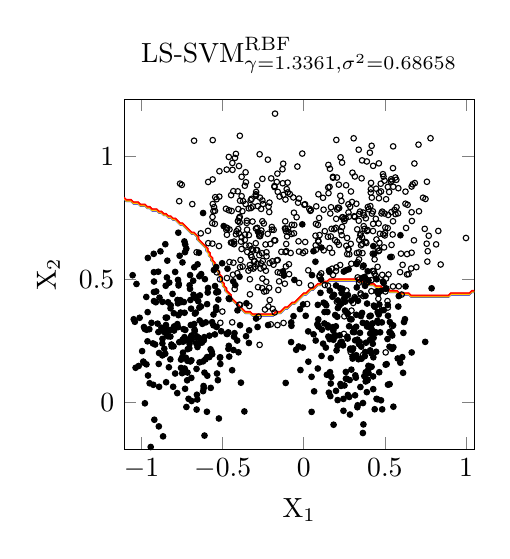
\begin{tikzpicture}

\begin{axis}[%
width=1.75in,
height=1.75in,
scale only axis,
xmin=-1.1078046378,
xmax=1.0502917026,
xlabel={$\text{X}_{\text{1}}$},
ymin=-0.18966497445,
ymax=1.2337404387,
ylabel={$\text{X}_{\text{2}}$},
title={$\text{LS-SVM}_{\gamma\text{=1.3361,}\sigma{}^\text{2}\text{=0.68658}}^{\text{RBF}}$}
]
\addplot[contour prepared, contour prepared format=matlab, contour/labels=false] table[row sep=crcr] {%
%
-0.8	225\\
-1.1078046378	0.8266464905391\\
-1.1063659069064	0.825697553597\\
-1.093417328864	0.8171571211181\\
-1.079030019928	0.8171571211181\\
-1.064642710992	0.8171571211181\\
-1.0632039800984	0.816208184176\\
-1.050255402056	0.8076677516971\\
-1.03586809312	0.8076677516971\\
-1.021480784184	0.8076677516971\\
-1.0200420532904	0.806718814755\\
-1.007093475248	0.7981783822761\\
-0.992706166312	0.7981783822761\\
-0.978318857376	0.7981783822761\\
-0.9768801264824	0.797229445334\\
-0.96393154844	0.7886890128551\\
-0.949544239504	0.7886890128551\\
-0.9481055086104	0.787740075913\\
-0.935156930568	0.7791996434341\\
-0.920769621632	0.7791996434341\\
-0.906382312696	0.7791996434341\\
-0.9049435818024	0.778250706492\\
-0.89199500376	0.7697102740131\\
-0.877607694824	0.7697102740131\\
-0.8761689639304	0.768761337071\\
-0.863220385888	0.7602209045921\\
-0.848833076952	0.7602209045921\\
-0.8473943460584	0.75927196765\\
-0.834445768016	0.7507315351711\\
-0.82005845908	0.7507315351711\\
-0.8186197281864	0.749782598229\\
-0.805671150144	0.7412421657501\\
-0.791283841208	0.7412421657501\\
-0.7898451103144	0.740293228808\\
-0.776896532272	0.7317527963291\\
-0.7754578013784	0.730803859387\\
-0.762509223336	0.7222634269081\\
-0.7481219144	0.7222634269081\\
-0.7466831835064	0.721314489966\\
-0.733734605464	0.7127740574871\\
-0.7322958745704	0.711825120545\\
-0.719347296528	0.7032846880661\\
-0.7179085656344	0.702335751124\\
-0.704959987592	0.6937953186451\\
-0.7035212566984	0.692846381703\\
-0.690572678656	0.6843059492241\\
-0.67618536972	0.6843059492241\\
-0.6747466388264	0.683357012282\\
-0.661798060784	0.6748165798031\\
-0.6603593298904	0.673867642861\\
-0.6603593298904	0.66437827344\\
-0.647410751848	0.6558378409611\\
-0.6459720209544	0.654888904019\\
-0.633023442912	0.6463484715401\\
-0.6315847120184	0.645399534598\\
-0.618636133976	0.6368591021191\\
-0.6171974030824	0.635910165177\\
-0.60424882504	0.6273697326981\\
-0.6028100941464	0.626420795756\\
-0.6028100941464	0.616931426335\\
-0.589861516104	0.6083909938561\\
-0.5884227852104	0.607442056914\\
-0.5884227852104	0.597952687493\\
-0.575474207168	0.5894122550141\\
-0.5740354762744	0.588463318072\\
-0.5740354762744	0.578973948651\\
-0.561086898232	0.5704335161721\\
-0.5596481673384	0.56948457923\\
-0.5596481673384	0.559995209809\\
-0.546699589296	0.5514547773301\\
-0.5452608584024	0.550505840388\\
-0.5452608584024	0.541016470967\\
-0.53231228036	0.5324760384881\\
-0.5308735494664	0.531527101546\\
-0.5308735494664	0.522037732125\\
-0.517924971424	0.5134972996461\\
-0.5164862405304	0.512548362704\\
-0.5164862405304	0.503058993283\\
-0.5164862405304	0.493569623862\\
-0.503537662488	0.4850291913831\\
-0.5020989315944	0.484080254441\\
-0.5020989315944	0.47459088502\\
-0.489150353552	0.4660504525411\\
-0.4877116226584	0.465101515599\\
-0.4877116226584	0.455612146178\\
-0.474763044616	0.4470717136991\\
-0.4733243137224	0.446122776757\\
-0.46037573568	0.4375823442781\\
-0.4589370047864	0.436633407336\\
-0.4589370047864	0.427144037915\\
-0.445988426744	0.4186036054361\\
-0.4445496958504	0.417654668494\\
-0.431601117808	0.4091142360151\\
-0.4301623869144	0.408165299073\\
-0.417213808872	0.3996248665941\\
-0.4157750779784	0.398675929652\\
-0.402826499936	0.3901354971731\\
-0.4013877690424	0.389186560231\\
-0.388439191	0.3806461277521\\
-0.3870004601064	0.37969719081\\
-0.374051882064	0.3711567583311\\
-0.3726131511704	0.370207821389\\
-0.359664573128	0.3616673889101\\
-0.345277264192	0.3616673889101\\
-0.330889955256	0.3616673889101\\
-0.3294512243624	0.360718451968\\
-0.31650264632	0.3521780194891\\
-0.302115337384	0.3521780194891\\
-0.287728028448	0.3521780194891\\
-0.273340719512	0.3521780194891\\
-0.258953410576	0.3521780194891\\
-0.24456610164	0.3521780194891\\
-0.230178792704	0.3521780194891\\
-0.215791483768	0.3521780194891\\
-0.201404174832	0.3521780194891\\
-0.187016865896	0.3521780194891\\
-0.1740682878536	0.360718451968\\
-0.17262955696	0.3616673889101\\
-0.158242248024	0.3616673889101\\
-0.143854939088	0.3616673889101\\
-0.1309063610456	0.370207821389\\
-0.129467630152	0.3711567583311\\
-0.1165190521096	0.37969719081\\
-0.115080321216	0.3806461277521\\
-0.10069301228	0.3806461277521\\
-0.0877444342375998	0.389186560231\\
-0.0863057033439998	0.3901354971731\\
-0.0733571253015999	0.398675929652\\
-0.071918394408	0.3996248665941\\
-0.0575310854719999	0.3996248665941\\
-0.0445825074295999	0.408165299073\\
-0.0431437765359999	0.4091142360151\\
-0.0301951984935998	0.417654668494\\
-0.0287564675999998	0.4186036054361\\
-0.0158078895575998	0.427144037915\\
-0.0143691586639998	0.4280929748571\\
-0.00142058062159975	0.436633407336\\
1.81502720002502e-05	0.4375823442781\\
0.0144054592080003	0.4375823442781\\
0.0273540372504001	0.446122776757\\
0.0287927681440001	0.4470717136991\\
0.0417413461864002	0.455612146178\\
0.0431800770800002	0.4565610831201\\
0.0575673860160002	0.4565610831201\\
0.0705159640584002	0.465101515599\\
0.0719546949520002	0.4660504525411\\
0.0849032729944002	0.47459088502\\
0.0863420038880002	0.4755398219621\\
0.100729312824	0.4755398219621\\
0.1136778908664	0.484080254441\\
0.11511662176	0.4850291913831\\
0.129503930696	0.4850291913831\\
0.143891239632	0.4850291913831\\
0.1568398176744	0.493569623862\\
0.158278548568	0.4945185608041\\
0.172665857504	0.4945185608041\\
0.18705316644	0.4945185608041\\
0.201440475376	0.4945185608041\\
0.215827784312	0.4945185608041\\
0.230215093248	0.4945185608041\\
0.244602402184	0.4945185608041\\
0.25898971112	0.4945185608041\\
0.273377020056	0.4945185608041\\
0.287764328992	0.4945185608041\\
0.302151637928	0.4945185608041\\
0.316538946864	0.4945185608041\\
0.3309262558	0.4945185608041\\
0.3323649866936	0.493569623862\\
0.345313564736	0.4850291913831\\
0.359700873672	0.4850291913831\\
0.374088182608	0.4850291913831\\
0.388475491544	0.4850291913831\\
0.3899142224376	0.484080254441\\
0.40286280048	0.4755398219621\\
0.417250109416	0.4755398219621\\
0.431637418352	0.4755398219621\\
0.4330761492456	0.47459088502\\
0.446024727288	0.4660504525411\\
0.460412036224	0.4660504525411\\
0.47479934516	0.4660504525411\\
0.4762380760536	0.465101515599\\
0.489186654096	0.4565610831201\\
0.503573963032	0.4565610831201\\
0.517961271968	0.4565610831201\\
0.5194000028616	0.455612146178\\
0.532348580904	0.4470717136991\\
0.54673588984	0.4470717136991\\
0.561123198776	0.4470717136991\\
0.575510507712	0.4470717136991\\
0.5769492386056	0.446122776757\\
0.589897816648	0.4375823442781\\
0.604285125584	0.4375823442781\\
0.61867243452	0.4375823442781\\
0.633059743456	0.4375823442781\\
0.647447052392	0.4375823442781\\
0.6488857832856	0.436633407336\\
0.661834361328	0.4280929748571\\
0.676221670264	0.4280929748571\\
0.6906089792	0.4280929748571\\
0.704996288136	0.4280929748571\\
0.719383597072	0.4280929748571\\
0.733770906008	0.4280929748571\\
0.748158214944	0.4280929748571\\
0.76254552388	0.4280929748571\\
0.776932832816	0.4280929748571\\
0.791320141752	0.4280929748571\\
0.805707450688	0.4280929748571\\
0.820094759624	0.4280929748571\\
0.83448206856	0.4280929748571\\
0.848869377496	0.4280929748571\\
0.863256686432	0.4280929748571\\
0.877643995368	0.4280929748571\\
0.892031304304	0.4280929748571\\
0.9049798823464	0.436633407336\\
0.90641861324	0.4375823442781\\
0.920805922176	0.4375823442781\\
0.935193231112	0.4375823442781\\
0.949580540048	0.4375823442781\\
0.963967848984	0.4375823442781\\
0.97835515792	0.4375823442781\\
0.992742466856	0.4375823442781\\
1.007129775792	0.4375823442781\\
1.021517084728	0.4375823442781\\
1.0344656627704	0.446122776757\\
1.035904393664	0.4470717136991\\
1.0502917026	0.4470717136991\\
-0.6	225\\
-1.1078046378	0.8275954274812\\
-1.1049271760128	0.825697553597\\
-1.093417328864	0.8181060580602\\
-1.079030019928	0.8181060580602\\
-1.064642710992	0.8181060580602\\
-1.0617652492048	0.816208184176\\
-1.050255402056	0.8086166886392\\
-1.03586809312	0.8086166886392\\
-1.021480784184	0.8086166886392\\
-1.0186033223968	0.806718814755\\
-1.007093475248	0.7991273192182\\
-0.992706166312	0.7991273192182\\
-0.978318857376	0.7991273192182\\
-0.9754413955888	0.797229445334\\
-0.96393154844	0.7896379497972\\
-0.949544239504	0.7896379497972\\
-0.9466667777168	0.787740075913\\
-0.935156930568	0.7801485803762\\
-0.920769621632	0.7801485803762\\
-0.906382312696	0.7801485803762\\
-0.9035048509088	0.778250706492\\
-0.89199500376	0.7706592109552\\
-0.877607694824	0.7706592109552\\
-0.8747302330368	0.768761337071\\
-0.863220385888	0.7611698415342\\
-0.848833076952	0.7611698415342\\
-0.8459556151648	0.75927196765\\
-0.834445768016	0.7516804721132\\
-0.82005845908	0.7516804721132\\
-0.8171809972928	0.749782598229\\
-0.805671150144	0.7421911026922\\
-0.791283841208	0.7421911026922\\
-0.7884063794208	0.740293228808\\
-0.776896532272	0.7327017332712\\
-0.7740190704848	0.730803859387\\
-0.762509223336	0.7232123638502\\
-0.7481219144	0.7232123638502\\
-0.7452444526128	0.721314489966\\
-0.733734605464	0.7137229944292\\
-0.7308571436768	0.711825120545\\
-0.719347296528	0.7042336250082\\
-0.7164698347408	0.702335751124\\
-0.704959987592	0.6947442555872\\
-0.7020825258048	0.692846381703\\
-0.690572678656	0.6852548861662\\
-0.67618536972	0.6852548861662\\
-0.6733079079328	0.683357012282\\
-0.661798060784	0.6757655167452\\
-0.6589205989968	0.673867642861\\
-0.6589205989968	0.66437827344\\
-0.647410751848	0.6567867779032\\
-0.6445332900608	0.654888904019\\
-0.633023442912	0.6472974084822\\
-0.6301459811248	0.645399534598\\
-0.618636133976	0.6378080390612\\
-0.6157586721888	0.635910165177\\
-0.60424882504	0.6283186696402\\
-0.6013713632528	0.626420795756\\
-0.6013713632528	0.616931426335\\
-0.589861516104	0.6093399307982\\
-0.5869840543168	0.607442056914\\
-0.5869840543168	0.597952687493\\
-0.575474207168	0.5903611919562\\
-0.5725967453808	0.588463318072\\
-0.5725967453808	0.578973948651\\
-0.561086898232	0.5713824531142\\
-0.5582094364448	0.56948457923\\
-0.5582094364448	0.559995209809\\
-0.546699589296	0.5524037142722\\
-0.5438221275088	0.550505840388\\
-0.5438221275088	0.541016470967\\
-0.53231228036	0.5334249754302\\
-0.5294348185728	0.531527101546\\
-0.5294348185728	0.522037732125\\
-0.517924971424	0.5144462365882\\
-0.5150475096368	0.512548362704\\
-0.5150475096368	0.503058993283\\
-0.5150475096368	0.493569623862\\
-0.503537662488	0.4859781283252\\
-0.5006602007008	0.484080254441\\
-0.5006602007008	0.47459088502\\
-0.489150353552	0.4669993894832\\
-0.4862728917648	0.465101515599\\
-0.4862728917648	0.455612146178\\
-0.474763044616	0.4480206506412\\
-0.4718855828288	0.446122776757\\
-0.46037573568	0.4385312812202\\
-0.4574982738928	0.436633407336\\
-0.4574982738928	0.427144037915\\
-0.445988426744	0.4195525423782\\
-0.4431109649568	0.417654668494\\
-0.431601117808	0.4100631729572\\
-0.4287236560208	0.408165299073\\
-0.417213808872	0.4005738035362\\
-0.4143363470848	0.398675929652\\
-0.402826499936	0.3910844341152\\
-0.3999490381488	0.389186560231\\
-0.388439191	0.3815950646942\\
-0.3855617292128	0.37969719081\\
-0.374051882064	0.3721056952732\\
-0.3711744202768	0.370207821389\\
-0.359664573128	0.3626163258522\\
-0.345277264192	0.3626163258522\\
-0.330889955256	0.3626163258522\\
-0.3280124934688	0.360718451968\\
-0.31650264632	0.3531269564312\\
-0.302115337384	0.3531269564312\\
-0.287728028448	0.3531269564312\\
-0.273340719512	0.3531269564312\\
-0.258953410576	0.3531269564312\\
-0.24456610164	0.3531269564312\\
-0.230178792704	0.3531269564312\\
-0.215791483768	0.3531269564312\\
-0.201404174832	0.3531269564312\\
-0.187016865896	0.3531269564312\\
-0.1755070187472	0.360718451968\\
-0.17262955696	0.3626163258522\\
-0.158242248024	0.3626163258522\\
-0.143854939088	0.3626163258522\\
-0.1323450919392	0.370207821389\\
-0.129467630152	0.3721056952732\\
-0.1179577830032	0.37969719081\\
-0.115080321216	0.3815950646942\\
-0.10069301228	0.3815950646942\\
-0.0891831651311998	0.389186560231\\
-0.0863057033439998	0.3910844341152\\
-0.0747958561951999	0.398675929652\\
-0.071918394408	0.4005738035362\\
-0.0575310854719999	0.4005738035362\\
-0.0460212383231999	0.408165299073\\
-0.0431437765359999	0.4100631729572\\
-0.0316339293871998	0.417654668494\\
-0.0287564675999998	0.4195525423782\\
-0.0172466204511998	0.427144037915\\
-0.0143691586639998	0.4290419117992\\
-0.00285931151519976	0.436633407336\\
1.81502720002502e-05	0.4385312812202\\
0.0144054592080003	0.4385312812202\\
0.0259153063568002	0.446122776757\\
0.0287927681440001	0.4480206506412\\
0.0403026152928001	0.455612146178\\
0.0431800770800002	0.4575100200622\\
0.0575673860160002	0.4575100200622\\
0.0690772331648002	0.465101515599\\
0.0719546949520002	0.4669993894832\\
0.0834645421008002	0.47459088502\\
0.0863420038880002	0.4764887589042\\
0.100729312824	0.4764887589042\\
0.1122391599728	0.484080254441\\
0.11511662176	0.4859781283252\\
0.129503930696	0.4859781283252\\
0.143891239632	0.4859781283252\\
0.1554010867808	0.493569623862\\
0.158278548568	0.4954674977462\\
0.172665857504	0.4954674977462\\
0.18705316644	0.4954674977462\\
0.201440475376	0.4954674977462\\
0.215827784312	0.4954674977462\\
0.230215093248	0.4954674977462\\
0.244602402184	0.4954674977462\\
0.25898971112	0.4954674977462\\
0.273377020056	0.4954674977462\\
0.287764328992	0.4954674977462\\
0.302151637928	0.4954674977462\\
0.316538946864	0.4954674977462\\
0.3309262558	0.4954674977462\\
0.3338037175872	0.493569623862\\
0.345313564736	0.4859781283252\\
0.359700873672	0.4859781283252\\
0.374088182608	0.4859781283252\\
0.388475491544	0.4859781283252\\
0.3913529533312	0.484080254441\\
0.40286280048	0.4764887589042\\
0.417250109416	0.4764887589042\\
0.431637418352	0.4764887589042\\
0.4345148801392	0.47459088502\\
0.446024727288	0.4669993894832\\
0.460412036224	0.4669993894832\\
0.47479934516	0.4669993894832\\
0.4776768069472	0.465101515599\\
0.489186654096	0.4575100200622\\
0.503573963032	0.4575100200622\\
0.517961271968	0.4575100200622\\
0.5208387337552	0.455612146178\\
0.532348580904	0.4480206506412\\
0.54673588984	0.4480206506412\\
0.561123198776	0.4480206506412\\
0.575510507712	0.4480206506412\\
0.5783879694992	0.446122776757\\
0.589897816648	0.4385312812202\\
0.604285125584	0.4385312812202\\
0.61867243452	0.4385312812202\\
0.633059743456	0.4385312812202\\
0.647447052392	0.4385312812202\\
0.6503245141792	0.436633407336\\
0.661834361328	0.4290419117992\\
0.676221670264	0.4290419117992\\
0.6906089792	0.4290419117992\\
0.704996288136	0.4290419117992\\
0.719383597072	0.4290419117992\\
0.733770906008	0.4290419117992\\
0.748158214944	0.4290419117992\\
0.76254552388	0.4290419117992\\
0.776932832816	0.4290419117992\\
0.791320141752	0.4290419117992\\
0.805707450688	0.4290419117992\\
0.820094759624	0.4290419117992\\
0.83448206856	0.4290419117992\\
0.848869377496	0.4290419117992\\
0.863256686432	0.4290419117992\\
0.877643995368	0.4290419117992\\
0.892031304304	0.4290419117992\\
0.9035411514528	0.436633407336\\
0.90641861324	0.4385312812202\\
0.920805922176	0.4385312812202\\
0.935193231112	0.4385312812202\\
0.949580540048	0.4385312812202\\
0.963967848984	0.4385312812202\\
0.97835515792	0.4385312812202\\
0.992742466856	0.4385312812202\\
1.007129775792	0.4385312812202\\
1.021517084728	0.4385312812202\\
1.0330269318768	0.446122776757\\
1.035904393664	0.4480206506412\\
1.0502917026	0.4480206506412\\
-0.4	225\\
-1.1078046378	0.8285443644233\\
-1.1034884451192	0.825697553597\\
-1.093417328864	0.8190549950023\\
-1.079030019928	0.8190549950023\\
-1.064642710992	0.8190549950023\\
-1.0603265183112	0.816208184176\\
-1.050255402056	0.8095656255813\\
-1.03586809312	0.8095656255813\\
-1.021480784184	0.8095656255813\\
-1.0171645915032	0.806718814755\\
-1.007093475248	0.8000762561603\\
-0.992706166312	0.8000762561603\\
-0.978318857376	0.8000762561603\\
-0.9740026646952	0.797229445334\\
-0.96393154844	0.7905868867393\\
-0.949544239504	0.7905868867393\\
-0.9452280468232	0.787740075913\\
-0.935156930568	0.7810975173183\\
-0.920769621632	0.7810975173183\\
-0.906382312696	0.7810975173183\\
-0.9020661200152	0.778250706492\\
-0.89199500376	0.7716081478973\\
-0.877607694824	0.7716081478973\\
-0.8732915021432	0.768761337071\\
-0.863220385888	0.7621187784763\\
-0.848833076952	0.7621187784763\\
-0.8445168842712	0.75927196765\\
-0.834445768016	0.7526294090553\\
-0.82005845908	0.7526294090553\\
-0.8157422663992	0.749782598229\\
-0.805671150144	0.7431400396343\\
-0.791283841208	0.7431400396343\\
-0.7869676485272	0.740293228808\\
-0.776896532272	0.7336506702133\\
-0.7725803395912	0.730803859387\\
-0.762509223336	0.7241613007923\\
-0.7481219144	0.7241613007923\\
-0.7438057217192	0.721314489966\\
-0.733734605464	0.7146719313713\\
-0.7294184127832	0.711825120545\\
-0.719347296528	0.7051825619503\\
-0.7150311038472	0.702335751124\\
-0.704959987592	0.6956931925293\\
-0.7006437949112	0.692846381703\\
-0.690572678656	0.6862038231083\\
-0.67618536972	0.6862038231083\\
-0.6718691770392	0.683357012282\\
-0.661798060784	0.6767144536873\\
-0.6574818681032	0.673867642861\\
-0.6574818681032	0.66437827344\\
-0.647410751848	0.6577357148453\\
-0.6430945591672	0.654888904019\\
-0.633023442912	0.6482463454243\\
-0.6287072502312	0.645399534598\\
-0.618636133976	0.6387569760033\\
-0.6143199412952	0.635910165177\\
-0.60424882504	0.6292676065823\\
-0.5999326323592	0.626420795756\\
-0.5999326323592	0.616931426335\\
-0.589861516104	0.6102888677403\\
-0.5855453234232	0.607442056914\\
-0.5855453234232	0.597952687493\\
-0.575474207168	0.5913101288983\\
-0.5711580144872	0.588463318072\\
-0.5711580144872	0.578973948651\\
-0.561086898232	0.5723313900563\\
-0.5567707055512	0.56948457923\\
-0.5567707055512	0.559995209809\\
-0.546699589296	0.5533526512143\\
-0.5423833966152	0.550505840388\\
-0.5423833966152	0.541016470967\\
-0.53231228036	0.5343739123723\\
-0.5279960876792	0.531527101546\\
-0.5279960876792	0.522037732125\\
-0.517924971424	0.5153951735303\\
-0.5136087787432	0.512548362704\\
-0.5136087787432	0.503058993283\\
-0.5136087787432	0.493569623862\\
-0.503537662488	0.4869270652673\\
-0.4992214698072	0.484080254441\\
-0.4992214698072	0.47459088502\\
-0.489150353552	0.4679483264253\\
-0.4848341608712	0.465101515599\\
-0.4848341608712	0.455612146178\\
-0.474763044616	0.4489695875833\\
-0.4704468519352	0.446122776757\\
-0.46037573568	0.4394802181623\\
-0.4560595429992	0.436633407336\\
-0.4560595429992	0.427144037915\\
-0.445988426744	0.4205014793203\\
-0.4416722340632	0.417654668494\\
-0.431601117808	0.4110121098993\\
-0.4272849251272	0.408165299073\\
-0.417213808872	0.4015227404783\\
-0.4128976161912	0.398675929652\\
-0.402826499936	0.3920333710573\\
-0.3985103072552	0.389186560231\\
-0.388439191	0.3825440016363\\
-0.3841229983192	0.37969719081\\
-0.374051882064	0.3730546322153\\
-0.3697356893832	0.370207821389\\
-0.359664573128	0.3635652627943\\
-0.345277264192	0.3635652627943\\
-0.330889955256	0.3635652627943\\
-0.3265737625752	0.360718451968\\
-0.31650264632	0.3540758933733\\
-0.302115337384	0.3540758933733\\
-0.287728028448	0.3540758933733\\
-0.273340719512	0.3540758933733\\
-0.258953410576	0.3540758933733\\
-0.24456610164	0.3540758933733\\
-0.230178792704	0.3540758933733\\
-0.215791483768	0.3540758933733\\
-0.201404174832	0.3540758933733\\
-0.187016865896	0.3540758933733\\
-0.1769457496408	0.360718451968\\
-0.17262955696	0.3635652627943\\
-0.158242248024	0.3635652627943\\
-0.143854939088	0.3635652627943\\
-0.1337838228328	0.370207821389\\
-0.129467630152	0.3730546322153\\
-0.1193965138968	0.37969719081\\
-0.115080321216	0.3825440016363\\
-0.10069301228	0.3825440016363\\
-0.0906218960247998	0.389186560231\\
-0.0863057033439998	0.3920333710573\\
-0.0762345870887999	0.398675929652\\
-0.071918394408	0.4015227404783\\
-0.0575310854719999	0.4015227404783\\
-0.0474599692167999	0.408165299073\\
-0.0431437765359999	0.4110121098993\\
-0.0330726602807998	0.417654668494\\
-0.0287564675999998	0.4205014793203\\
-0.0186853513447998	0.427144037915\\
-0.0143691586639998	0.4299908487413\\
-0.00429804240879976	0.436633407336\\
1.81502720002502e-05	0.4394802181623\\
0.0144054592080003	0.4394802181623\\
0.0244765754632002	0.446122776757\\
0.0287927681440001	0.4489695875833\\
0.0388638843992001	0.455612146178\\
0.0431800770800002	0.4584589570043\\
0.0575673860160002	0.4584589570043\\
0.0676385022712002	0.465101515599\\
0.0719546949520002	0.4679483264253\\
0.0820258112072002	0.47459088502\\
0.0863420038880002	0.4774376958463\\
0.100729312824	0.4774376958463\\
0.1108004290792	0.484080254441\\
0.11511662176	0.4869270652673\\
0.129503930696	0.4869270652673\\
0.143891239632	0.4869270652673\\
0.1539623558872	0.493569623862\\
0.158278548568	0.4964164346883\\
0.172665857504	0.4964164346883\\
0.18705316644	0.4964164346883\\
0.201440475376	0.4964164346883\\
0.215827784312	0.4964164346883\\
0.230215093248	0.4964164346883\\
0.244602402184	0.4964164346883\\
0.25898971112	0.4964164346883\\
0.273377020056	0.4964164346883\\
0.287764328992	0.4964164346883\\
0.302151637928	0.4964164346883\\
0.316538946864	0.4964164346883\\
0.3309262558	0.4964164346883\\
0.3352424484808	0.493569623862\\
0.345313564736	0.4869270652673\\
0.359700873672	0.4869270652673\\
0.374088182608	0.4869270652673\\
0.388475491544	0.4869270652673\\
0.3927916842248	0.484080254441\\
0.40286280048	0.4774376958463\\
0.417250109416	0.4774376958463\\
0.431637418352	0.4774376958463\\
0.4359536110328	0.47459088502\\
0.446024727288	0.4679483264253\\
0.460412036224	0.4679483264253\\
0.47479934516	0.4679483264253\\
0.4791155378408	0.465101515599\\
0.489186654096	0.4584589570043\\
0.503573963032	0.4584589570043\\
0.517961271968	0.4584589570043\\
0.5222774646488	0.455612146178\\
0.532348580904	0.4489695875833\\
0.54673588984	0.4489695875833\\
0.561123198776	0.4489695875833\\
0.575510507712	0.4489695875833\\
0.5798267003928	0.446122776757\\
0.589897816648	0.4394802181623\\
0.604285125584	0.4394802181623\\
0.61867243452	0.4394802181623\\
0.633059743456	0.4394802181623\\
0.647447052392	0.4394802181623\\
0.6517632450728	0.436633407336\\
0.661834361328	0.4299908487413\\
0.676221670264	0.4299908487413\\
0.6906089792	0.4299908487413\\
0.704996288136	0.4299908487413\\
0.719383597072	0.4299908487413\\
0.733770906008	0.4299908487413\\
0.748158214944	0.4299908487413\\
0.76254552388	0.4299908487413\\
0.776932832816	0.4299908487413\\
0.791320141752	0.4299908487413\\
0.805707450688	0.4299908487413\\
0.820094759624	0.4299908487413\\
0.83448206856	0.4299908487413\\
0.848869377496	0.4299908487413\\
0.863256686432	0.4299908487413\\
0.877643995368	0.4299908487413\\
0.892031304304	0.4299908487413\\
0.9021024205592	0.436633407336\\
0.90641861324	0.4394802181623\\
0.920805922176	0.4394802181623\\
0.935193231112	0.4394802181623\\
0.949580540048	0.4394802181623\\
0.963967848984	0.4394802181623\\
0.97835515792	0.4394802181623\\
0.992742466856	0.4394802181623\\
1.007129775792	0.4394802181623\\
1.021517084728	0.4394802181623\\
1.0315882009832	0.446122776757\\
1.035904393664	0.4489695875833\\
1.0502917026	0.4489695875833\\
-0.2	225\\
-1.1078046378	0.8294933013654\\
-1.1020497142256	0.825697553597\\
-1.093417328864	0.8200039319444\\
-1.079030019928	0.8200039319444\\
-1.064642710992	0.8200039319444\\
-1.0588877874176	0.816208184176\\
-1.050255402056	0.8105145625234\\
-1.03586809312	0.8105145625234\\
-1.021480784184	0.8105145625234\\
-1.0157258606096	0.806718814755\\
-1.007093475248	0.8010251931024\\
-0.992706166312	0.8010251931024\\
-0.978318857376	0.8010251931024\\
-0.9725639338016	0.797229445334\\
-0.96393154844	0.7915358236814\\
-0.949544239504	0.7915358236814\\
-0.9437893159296	0.787740075913\\
-0.935156930568	0.7820464542604\\
-0.920769621632	0.7820464542604\\
-0.906382312696	0.7820464542604\\
-0.9006273891216	0.778250706492\\
-0.89199500376	0.7725570848394\\
-0.877607694824	0.7725570848394\\
-0.8718527712496	0.768761337071\\
-0.863220385888	0.7630677154184\\
-0.848833076952	0.7630677154184\\
-0.8430781533776	0.75927196765\\
-0.834445768016	0.7535783459974\\
-0.82005845908	0.7535783459974\\
-0.8143035355056	0.749782598229\\
-0.805671150144	0.7440889765764\\
-0.791283841208	0.7440889765764\\
-0.7855289176336	0.740293228808\\
-0.776896532272	0.7345996071554\\
-0.7711416086976	0.730803859387\\
-0.762509223336	0.7251102377344\\
-0.7481219144	0.7251102377344\\
-0.7423669908256	0.721314489966\\
-0.733734605464	0.7156208683134\\
-0.7279796818896	0.711825120545\\
-0.719347296528	0.7061314988924\\
-0.7135923729536	0.702335751124\\
-0.704959987592	0.6966421294714\\
-0.6992050640176	0.692846381703\\
-0.690572678656	0.6871527600504\\
-0.67618536972	0.6871527600504\\
-0.6704304461456	0.683357012282\\
-0.661798060784	0.6776633906294\\
-0.6560431372096	0.673867642861\\
-0.6560431372096	0.66437827344\\
-0.647410751848	0.6586846517874\\
-0.6416558282736	0.654888904019\\
-0.633023442912	0.6491952823664\\
-0.6272685193376	0.645399534598\\
-0.618636133976	0.6397059129454\\
-0.6128812104016	0.635910165177\\
-0.60424882504	0.6302165435244\\
-0.5984939014656	0.626420795756\\
-0.5984939014656	0.616931426335\\
-0.589861516104	0.6112378046824\\
-0.5841065925296	0.607442056914\\
-0.5841065925296	0.597952687493\\
-0.575474207168	0.5922590658404\\
-0.5697192835936	0.588463318072\\
-0.5697192835936	0.578973948651\\
-0.561086898232	0.5732803269984\\
-0.5553319746576	0.56948457923\\
-0.5553319746576	0.559995209809\\
-0.546699589296	0.5543015881564\\
-0.5409446657216	0.550505840388\\
-0.5409446657216	0.541016470967\\
-0.53231228036	0.5353228493144\\
-0.5265573567856	0.531527101546\\
-0.5265573567856	0.522037732125\\
-0.517924971424	0.5163441104724\\
-0.5121700478496	0.512548362704\\
-0.5121700478496	0.503058993283\\
-0.5121700478496	0.493569623862\\
-0.503537662488	0.4878760022094\\
-0.4977827389136	0.484080254441\\
-0.4977827389136	0.47459088502\\
-0.489150353552	0.4688972633674\\
-0.4833954299776	0.465101515599\\
-0.4833954299776	0.455612146178\\
-0.474763044616	0.4499185245254\\
-0.4690081210416	0.446122776757\\
-0.46037573568	0.4404291551044\\
-0.4546208121056	0.436633407336\\
-0.4546208121056	0.427144037915\\
-0.445988426744	0.4214504162624\\
-0.4402335031696	0.417654668494\\
-0.431601117808	0.4119610468414\\
-0.4258461942336	0.408165299073\\
-0.417213808872	0.4024716774204\\
-0.4114588852976	0.398675929652\\
-0.402826499936	0.3929823079994\\
-0.3970715763616	0.389186560231\\
-0.388439191	0.3834929385784\\
-0.3826842674256	0.37969719081\\
-0.374051882064	0.3740035691574\\
-0.3682969584896	0.370207821389\\
-0.359664573128	0.3645141997364\\
-0.345277264192	0.3645141997364\\
-0.330889955256	0.3645141997364\\
-0.3251350316816	0.360718451968\\
-0.31650264632	0.3550248303154\\
-0.302115337384	0.3550248303154\\
-0.287728028448	0.3550248303154\\
-0.273340719512	0.3550248303154\\
-0.258953410576	0.3550248303154\\
-0.24456610164	0.3550248303154\\
-0.230178792704	0.3550248303154\\
-0.215791483768	0.3550248303154\\
-0.201404174832	0.3550248303154\\
-0.187016865896	0.3550248303154\\
-0.1783844805344	0.360718451968\\
-0.17262955696	0.3645141997364\\
-0.158242248024	0.3645141997364\\
-0.143854939088	0.3645141997364\\
-0.1352225537264	0.370207821389\\
-0.129467630152	0.3740035691574\\
-0.1208352447904	0.37969719081\\
-0.115080321216	0.3834929385784\\
-0.10069301228	0.3834929385784\\
-0.0920606269183998	0.389186560231\\
-0.0863057033439998	0.3929823079994\\
-0.0776733179823999	0.398675929652\\
-0.071918394408	0.4024716774204\\
-0.0575310854719999	0.4024716774204\\
-0.0488987001103999	0.408165299073\\
-0.0431437765359999	0.4119610468414\\
-0.0345113911743999	0.417654668494\\
-0.0287564675999998	0.4214504162624\\
-0.0201240822383998	0.427144037915\\
-0.0143691586639998	0.4309397856834\\
-0.00573677330239977	0.436633407336\\
1.81502720002502e-05	0.4404291551044\\
0.0144054592080003	0.4404291551044\\
0.0230378445696002	0.446122776757\\
0.0287927681440001	0.4499185245254\\
0.0374251535056001	0.455612146178\\
0.0431800770800002	0.4594078939464\\
0.0575673860160002	0.4594078939464\\
0.0661997713776002	0.465101515599\\
0.0719546949520002	0.4688972633674\\
0.0805870803136002	0.47459088502\\
0.0863420038880002	0.4783866327884\\
0.100729312824	0.4783866327884\\
0.1093616981856	0.484080254441\\
0.11511662176	0.4878760022094\\
0.129503930696	0.4878760022094\\
0.143891239632	0.4878760022094\\
0.1525236249936	0.493569623862\\
0.158278548568	0.4973653716304\\
0.172665857504	0.4973653716304\\
0.18705316644	0.4973653716304\\
0.201440475376	0.4973653716304\\
0.215827784312	0.4973653716304\\
0.230215093248	0.4973653716304\\
0.244602402184	0.4973653716304\\
0.25898971112	0.4973653716304\\
0.273377020056	0.4973653716304\\
0.287764328992	0.4973653716304\\
0.302151637928	0.4973653716304\\
0.316538946864	0.4973653716304\\
0.3309262558	0.4973653716304\\
0.3366811793744	0.493569623862\\
0.345313564736	0.4878760022094\\
0.359700873672	0.4878760022094\\
0.374088182608	0.4878760022094\\
0.388475491544	0.4878760022094\\
0.3942304151184	0.484080254441\\
0.40286280048	0.4783866327884\\
0.417250109416	0.4783866327884\\
0.431637418352	0.4783866327884\\
0.4373923419264	0.47459088502\\
0.446024727288	0.4688972633674\\
0.460412036224	0.4688972633674\\
0.47479934516	0.4688972633674\\
0.4805542687344	0.465101515599\\
0.489186654096	0.4594078939464\\
0.503573963032	0.4594078939464\\
0.517961271968	0.4594078939464\\
0.5237161955424	0.455612146178\\
0.532348580904	0.4499185245254\\
0.54673588984	0.4499185245254\\
0.561123198776	0.4499185245254\\
0.575510507712	0.4499185245254\\
0.5812654312864	0.446122776757\\
0.589897816648	0.4404291551044\\
0.604285125584	0.4404291551044\\
0.61867243452	0.4404291551044\\
0.633059743456	0.4404291551044\\
0.647447052392	0.4404291551044\\
0.6532019759664	0.436633407336\\
0.661834361328	0.4309397856834\\
0.676221670264	0.4309397856834\\
0.6906089792	0.4309397856834\\
0.704996288136	0.4309397856834\\
0.719383597072	0.4309397856834\\
0.733770906008	0.4309397856834\\
0.748158214944	0.4309397856834\\
0.76254552388	0.4309397856834\\
0.776932832816	0.4309397856834\\
0.791320141752	0.4309397856834\\
0.805707450688	0.4309397856834\\
0.820094759624	0.4309397856834\\
0.83448206856	0.4309397856834\\
0.848869377496	0.4309397856834\\
0.863256686432	0.4309397856834\\
0.877643995368	0.4309397856834\\
0.892031304304	0.4309397856834\\
0.9006636896656	0.436633407336\\
0.90641861324	0.4404291551044\\
0.920805922176	0.4404291551044\\
0.935193231112	0.4404291551044\\
0.949580540048	0.4404291551044\\
0.963967848984	0.4404291551044\\
0.97835515792	0.4404291551044\\
0.992742466856	0.4404291551044\\
1.007129775792	0.4404291551044\\
1.021517084728	0.4404291551044\\
1.0301494700896	0.446122776757\\
1.035904393664	0.4499185245254\\
1.0502917026	0.4499185245254\\
0	225\\
-1.1078046378	0.8304422383075\\
-1.100610983332	0.825697553597\\
-1.093417328864	0.8209528688865\\
-1.079030019928	0.8209528688865\\
-1.064642710992	0.8209528688865\\
-1.057449056524	0.816208184176\\
-1.050255402056	0.8114634994655\\
-1.03586809312	0.8114634994655\\
-1.021480784184	0.8114634994655\\
-1.014287129716	0.806718814755\\
-1.007093475248	0.8019741300445\\
-0.992706166312	0.8019741300445\\
-0.978318857376	0.8019741300445\\
-0.971125202908	0.797229445334\\
-0.96393154844	0.7924847606235\\
-0.949544239504	0.7924847606235\\
-0.942350585036	0.787740075913\\
-0.935156930568	0.7829953912025\\
-0.920769621632	0.7829953912025\\
-0.906382312696	0.7829953912025\\
-0.899188658228	0.778250706492\\
-0.89199500376	0.7735060217815\\
-0.877607694824	0.7735060217815\\
-0.870414040356	0.768761337071\\
-0.863220385888	0.7640166523605\\
-0.848833076952	0.7640166523605\\
-0.841639422484	0.75927196765\\
-0.834445768016	0.7545272829395\\
-0.82005845908	0.7545272829395\\
-0.812864804612	0.749782598229\\
-0.805671150144	0.7450379135185\\
-0.791283841208	0.7450379135185\\
-0.78409018674	0.740293228808\\
-0.776896532272	0.7355485440975\\
-0.769702877804	0.730803859387\\
-0.762509223336	0.7260591746765\\
-0.7481219144	0.7260591746765\\
-0.740928259932	0.721314489966\\
-0.733734605464	0.7165698052555\\
-0.726540950996	0.711825120545\\
-0.719347296528	0.7070804358345\\
-0.71215364206	0.702335751124\\
-0.704959987592	0.6975910664135\\
-0.697766333124	0.692846381703\\
-0.690572678656	0.6881016969925\\
-0.67618536972	0.6881016969925\\
-0.668991715252	0.683357012282\\
-0.661798060784	0.6786123275715\\
-0.654604406316	0.673867642861\\
-0.654604406316	0.66437827344\\
-0.647410751848	0.6596335887295\\
-0.64021709738	0.654888904019\\
-0.633023442912	0.6501442193085\\
-0.625829788444	0.645399534598\\
-0.618636133976	0.6406548498875\\
-0.611442479508	0.635910165177\\
-0.60424882504	0.6311654804665\\
-0.597055170572	0.626420795756\\
-0.597055170572	0.616931426335\\
-0.589861516104	0.6121867416245\\
-0.582667861636	0.607442056914\\
-0.582667861636	0.597952687493\\
-0.575474207168	0.5932080027825\\
-0.5682805527	0.588463318072\\
-0.5682805527	0.578973948651\\
-0.561086898232	0.5742292639405\\
-0.553893243764	0.56948457923\\
-0.553893243764	0.559995209809\\
-0.546699589296	0.5552505250985\\
-0.539505934828	0.550505840388\\
-0.539505934828	0.541016470967\\
-0.53231228036	0.5362717862565\\
-0.525118625892	0.531527101546\\
-0.525118625892	0.522037732125\\
-0.517924971424	0.5172930474145\\
-0.510731316956	0.512548362704\\
-0.510731316956	0.503058993283\\
-0.510731316956	0.493569623862\\
-0.503537662488	0.4888249391515\\
-0.49634400802	0.484080254441\\
-0.49634400802	0.47459088502\\
-0.489150353552	0.4698462003095\\
-0.481956699084	0.465101515599\\
-0.481956699084	0.455612146178\\
-0.474763044616	0.4508674614675\\
-0.467569390148	0.446122776757\\
-0.46037573568	0.4413780920465\\
-0.453182081212	0.436633407336\\
-0.453182081212	0.427144037915\\
-0.445988426744	0.4223993532045\\
-0.438794772276	0.417654668494\\
-0.431601117808	0.4129099837835\\
-0.42440746334	0.408165299073\\
-0.417213808872	0.4034206143625\\
-0.410020154404	0.398675929652\\
-0.402826499936	0.3939312449415\\
-0.395632845468	0.389186560231\\
-0.388439191	0.3844418755205\\
-0.381245536532	0.37969719081\\
-0.374051882064	0.3749525060995\\
-0.366858227596	0.370207821389\\
-0.359664573128	0.3654631366785\\
-0.345277264192	0.3654631366785\\
-0.330889955256	0.3654631366785\\
-0.323696300788	0.360718451968\\
-0.31650264632	0.3559737672575\\
-0.302115337384	0.3559737672575\\
-0.287728028448	0.3559737672575\\
-0.273340719512	0.3559737672575\\
-0.258953410576	0.3559737672575\\
-0.24456610164	0.3559737672575\\
-0.230178792704	0.3559737672575\\
-0.215791483768	0.3559737672575\\
-0.201404174832	0.3559737672575\\
-0.187016865896	0.3559737672575\\
-0.179823211428	0.360718451968\\
-0.17262955696	0.3654631366785\\
-0.158242248024	0.3654631366785\\
-0.143854939088	0.3654631366785\\
-0.13666128462	0.370207821389\\
-0.129467630152	0.3749525060995\\
-0.122273975684	0.37969719081\\
-0.115080321216	0.3844418755205\\
-0.10069301228	0.3844418755205\\
-0.0934993578119998	0.389186560231\\
-0.0863057033439998	0.3939312449415\\
-0.0791120488759999	0.398675929652\\
-0.071918394408	0.4034206143625\\
-0.0575310854719999	0.4034206143625\\
-0.0503374310039999	0.408165299073\\
-0.0431437765359999	0.4129099837835\\
-0.0359501220679999	0.417654668494\\
-0.0287564675999998	0.4223993532045\\
-0.0215628131319998	0.427144037915\\
-0.0143691586639998	0.4318887226255\\
-0.00717550419599977	0.436633407336\\
1.81502720002502e-05	0.4413780920465\\
0.0144054592080003	0.4413780920465\\
0.0215991136760002	0.446122776757\\
0.0287927681440001	0.4508674614675\\
0.0359864226120001	0.455612146178\\
0.0431800770800002	0.4603568308885\\
0.0575673860160002	0.4603568308885\\
0.0647610404840002	0.465101515599\\
0.0719546949520002	0.4698462003095\\
0.0791483494200002	0.47459088502\\
0.0863420038880002	0.4793355697305\\
0.100729312824	0.4793355697305\\
0.107922967292	0.484080254441\\
0.11511662176	0.4888249391515\\
0.129503930696	0.4888249391515\\
0.143891239632	0.4888249391515\\
0.1510848941	0.493569623862\\
0.158278548568	0.4983143085725\\
0.172665857504	0.4983143085725\\
0.18705316644	0.4983143085725\\
0.201440475376	0.4983143085725\\
0.215827784312	0.4983143085725\\
0.230215093248	0.4983143085725\\
0.244602402184	0.4983143085725\\
0.25898971112	0.4983143085725\\
0.273377020056	0.4983143085725\\
0.287764328992	0.4983143085725\\
0.302151637928	0.4983143085725\\
0.316538946864	0.4983143085725\\
0.3309262558	0.4983143085725\\
0.338119910268	0.493569623862\\
0.345313564736	0.4888249391515\\
0.359700873672	0.4888249391515\\
0.374088182608	0.4888249391515\\
0.388475491544	0.4888249391515\\
0.395669146012	0.484080254441\\
0.40286280048	0.4793355697305\\
0.417250109416	0.4793355697305\\
0.431637418352	0.4793355697305\\
0.43883107282	0.47459088502\\
0.446024727288	0.4698462003095\\
0.460412036224	0.4698462003095\\
0.47479934516	0.4698462003095\\
0.481992999628	0.465101515599\\
0.489186654096	0.4603568308885\\
0.503573963032	0.4603568308885\\
0.517961271968	0.4603568308885\\
0.525154926436	0.455612146178\\
0.532348580904	0.4508674614675\\
0.54673588984	0.4508674614675\\
0.561123198776	0.4508674614675\\
0.575510507712	0.4508674614675\\
0.58270416218	0.446122776757\\
0.589897816648	0.4413780920465\\
0.604285125584	0.4413780920465\\
0.61867243452	0.4413780920465\\
0.633059743456	0.4413780920465\\
0.647447052392	0.4413780920465\\
0.65464070686	0.436633407336\\
0.661834361328	0.4318887226255\\
0.676221670264	0.4318887226255\\
0.6906089792	0.4318887226255\\
0.704996288136	0.4318887226255\\
0.719383597072	0.4318887226255\\
0.733770906008	0.4318887226255\\
0.748158214944	0.4318887226255\\
0.76254552388	0.4318887226255\\
0.776932832816	0.4318887226255\\
0.791320141752	0.4318887226255\\
0.805707450688	0.4318887226255\\
0.820094759624	0.4318887226255\\
0.83448206856	0.4318887226255\\
0.848869377496	0.4318887226255\\
0.863256686432	0.4318887226255\\
0.877643995368	0.4318887226255\\
0.892031304304	0.4318887226255\\
0.899224958772	0.436633407336\\
0.90641861324	0.4413780920465\\
0.920805922176	0.4413780920465\\
0.935193231112	0.4413780920465\\
0.949580540048	0.4413780920465\\
0.963967848984	0.4413780920465\\
0.97835515792	0.4413780920465\\
0.992742466856	0.4413780920465\\
1.007129775792	0.4413780920465\\
1.021517084728	0.4413780920465\\
1.028710739196	0.446122776757\\
1.035904393664	0.4508674614675\\
1.0502917026	0.4508674614675\\
0.2	225\\
-1.1078046378	0.8313911752496\\
-1.0991722524384	0.825697553597\\
-1.093417328864	0.8219018058286\\
-1.079030019928	0.8219018058286\\
-1.064642710992	0.8219018058286\\
-1.0560103256304	0.816208184176\\
-1.050255402056	0.8124124364076\\
-1.03586809312	0.8124124364076\\
-1.021480784184	0.8124124364076\\
-1.0128483988224	0.806718814755\\
-1.007093475248	0.8029230669866\\
-0.992706166312	0.8029230669866\\
-0.978318857376	0.8029230669866\\
-0.9696864720144	0.797229445334\\
-0.96393154844	0.7934336975656\\
-0.949544239504	0.7934336975656\\
-0.9409118541424	0.787740075913\\
-0.935156930568	0.7839443281446\\
-0.920769621632	0.7839443281446\\
-0.906382312696	0.7839443281446\\
-0.8977499273344	0.778250706492\\
-0.89199500376	0.7744549587236\\
-0.877607694824	0.7744549587236\\
-0.8689753094624	0.768761337071\\
-0.863220385888	0.7649655893026\\
-0.848833076952	0.7649655893026\\
-0.8402006915904	0.75927196765\\
-0.834445768016	0.7554762198816\\
-0.82005845908	0.7554762198816\\
-0.8114260737184	0.749782598229\\
-0.805671150144	0.7459868504606\\
-0.791283841208	0.7459868504606\\
-0.7826514558464	0.740293228808\\
-0.776896532272	0.7364974810396\\
-0.7682641469104	0.730803859387\\
-0.762509223336	0.7270081116186\\
-0.7481219144	0.7270081116186\\
-0.7394895290384	0.721314489966\\
-0.733734605464	0.7175187421976\\
-0.7251022201024	0.711825120545\\
-0.719347296528	0.7080293727766\\
-0.7107149111664	0.702335751124\\
-0.704959987592	0.6985400033556\\
-0.6963276022304	0.692846381703\\
-0.690572678656	0.6890506339346\\
-0.67618536972	0.6890506339346\\
-0.6675529843584	0.683357012282\\
-0.661798060784	0.6795612645136\\
-0.6531656754224	0.673867642861\\
-0.6531656754224	0.66437827344\\
-0.647410751848	0.6605825256716\\
-0.6387783664864	0.654888904019\\
-0.633023442912	0.6510931562506\\
-0.6243910575504	0.645399534598\\
-0.618636133976	0.6416037868296\\
-0.6100037486144	0.635910165177\\
-0.60424882504	0.6321144174086\\
-0.5956164396784	0.626420795756\\
-0.5956164396784	0.616931426335\\
-0.589861516104	0.6131356785666\\
-0.5812291307424	0.607442056914\\
-0.5812291307424	0.597952687493\\
-0.575474207168	0.5941569397246\\
-0.5668418218064	0.588463318072\\
-0.5668418218064	0.578973948651\\
-0.561086898232	0.5751782008826\\
-0.5524545128704	0.56948457923\\
-0.5524545128704	0.559995209809\\
-0.546699589296	0.5561994620406\\
-0.5380672039344	0.550505840388\\
-0.5380672039344	0.541016470967\\
-0.53231228036	0.5372207231986\\
-0.5236798949984	0.531527101546\\
-0.5236798949984	0.522037732125\\
-0.517924971424	0.5182419843566\\
-0.5092925860624	0.512548362704\\
-0.5092925860624	0.503058993283\\
-0.5092925860624	0.493569623862\\
-0.503537662488	0.4897738760936\\
-0.4949052771264	0.484080254441\\
-0.4949052771264	0.47459088502\\
-0.489150353552	0.4707951372516\\
-0.4805179681904	0.465101515599\\
-0.4805179681904	0.455612146178\\
-0.474763044616	0.4518163984096\\
-0.4661306592544	0.446122776757\\
-0.46037573568	0.4423270289886\\
-0.4517433503184	0.436633407336\\
-0.4517433503184	0.427144037915\\
-0.445988426744	0.4233482901466\\
-0.4373560413824	0.417654668494\\
-0.431601117808	0.4138589207256\\
-0.4229687324464	0.408165299073\\
-0.417213808872	0.4043695513046\\
-0.4085814235104	0.398675929652\\
-0.402826499936	0.3948801818836\\
-0.3941941145744	0.389186560231\\
-0.388439191	0.3853908124626\\
-0.3798068056384	0.37969719081\\
-0.374051882064	0.3759014430416\\
-0.3654194967024	0.370207821389\\
-0.359664573128	0.3664120736206\\
-0.345277264192	0.3664120736206\\
-0.330889955256	0.3664120736206\\
-0.3222575698944	0.360718451968\\
-0.31650264632	0.3569227041996\\
-0.302115337384	0.3569227041996\\
-0.287728028448	0.3569227041996\\
-0.273340719512	0.3569227041996\\
-0.258953410576	0.3569227041996\\
-0.24456610164	0.3569227041996\\
-0.230178792704	0.3569227041996\\
-0.215791483768	0.3569227041996\\
-0.201404174832	0.3569227041996\\
-0.187016865896	0.3569227041996\\
-0.1812619423216	0.360718451968\\
-0.17262955696	0.3664120736206\\
-0.158242248024	0.3664120736206\\
-0.143854939088	0.3664120736206\\
-0.1381000155136	0.370207821389\\
-0.129467630152	0.3759014430416\\
-0.1237127065776	0.37969719081\\
-0.115080321216	0.3853908124626\\
-0.10069301228	0.3853908124626\\
-0.0949380887055998	0.389186560231\\
-0.0863057033439998	0.3948801818836\\
-0.0805507797695999	0.398675929652\\
-0.071918394408	0.4043695513046\\
-0.0575310854719999	0.4043695513046\\
-0.0517761618975999	0.408165299073\\
-0.0431437765359999	0.4138589207256\\
-0.0373888529615999	0.417654668494\\
-0.0287564675999998	0.4233482901466\\
-0.0230015440255998	0.427144037915\\
-0.0143691586639998	0.4328376595676\\
-0.00861423508959978	0.436633407336\\
1.81502720002502e-05	0.4423270289886\\
0.0144054592080003	0.4423270289886\\
0.0201603827824002	0.446122776757\\
0.0287927681440001	0.4518163984096\\
0.0345476917184001	0.455612146178\\
0.0431800770800002	0.4613057678306\\
0.0575673860160002	0.4613057678306\\
0.0633223095904002	0.465101515599\\
0.0719546949520002	0.4707951372516\\
0.0777096185264002	0.47459088502\\
0.0863420038880002	0.4802845066726\\
0.100729312824	0.4802845066726\\
0.1064842363984	0.484080254441\\
0.11511662176	0.4897738760936\\
0.129503930696	0.4897738760936\\
0.143891239632	0.4897738760936\\
0.1496461632064	0.493569623862\\
0.158278548568	0.4992632455146\\
0.172665857504	0.4992632455146\\
0.18705316644	0.4992632455146\\
0.201440475376	0.4992632455146\\
0.215827784312	0.4992632455146\\
0.230215093248	0.4992632455146\\
0.244602402184	0.4992632455146\\
0.25898971112	0.4992632455146\\
0.273377020056	0.4992632455146\\
0.287764328992	0.4992632455146\\
0.302151637928	0.4992632455146\\
0.316538946864	0.4992632455146\\
0.3309262558	0.4992632455146\\
0.3395586411616	0.493569623862\\
0.345313564736	0.4897738760936\\
0.359700873672	0.4897738760936\\
0.374088182608	0.4897738760936\\
0.388475491544	0.4897738760936\\
0.3971078769056	0.484080254441\\
0.40286280048	0.4802845066726\\
0.417250109416	0.4802845066726\\
0.431637418352	0.4802845066726\\
0.4402698037136	0.47459088502\\
0.446024727288	0.4707951372516\\
0.460412036224	0.4707951372516\\
0.47479934516	0.4707951372516\\
0.4834317305216	0.465101515599\\
0.489186654096	0.4613057678306\\
0.503573963032	0.4613057678306\\
0.517961271968	0.4613057678306\\
0.5265936573296	0.455612146178\\
0.532348580904	0.4518163984096\\
0.54673588984	0.4518163984096\\
0.561123198776	0.4518163984096\\
0.575510507712	0.4518163984096\\
0.5841428930736	0.446122776757\\
0.589897816648	0.4423270289886\\
0.604285125584	0.4423270289886\\
0.61867243452	0.4423270289886\\
0.633059743456	0.4423270289886\\
0.647447052392	0.4423270289886\\
0.6560794377536	0.436633407336\\
0.661834361328	0.4328376595676\\
0.676221670264	0.4328376595676\\
0.6906089792	0.4328376595676\\
0.704996288136	0.4328376595676\\
0.719383597072	0.4328376595676\\
0.733770906008	0.4328376595676\\
0.748158214944	0.4328376595676\\
0.76254552388	0.4328376595676\\
0.776932832816	0.4328376595676\\
0.791320141752	0.4328376595676\\
0.805707450688	0.4328376595676\\
0.820094759624	0.4328376595676\\
0.83448206856	0.4328376595676\\
0.848869377496	0.4328376595676\\
0.863256686432	0.4328376595676\\
0.877643995368	0.4328376595676\\
0.892031304304	0.4328376595676\\
0.8977862278784	0.436633407336\\
0.90641861324	0.4423270289886\\
0.920805922176	0.4423270289886\\
0.935193231112	0.4423270289886\\
0.949580540048	0.4423270289886\\
0.963967848984	0.4423270289886\\
0.97835515792	0.4423270289886\\
0.992742466856	0.4423270289886\\
1.007129775792	0.4423270289886\\
1.021517084728	0.4423270289886\\
1.0272720083024	0.446122776757\\
1.035904393664	0.4518163984096\\
1.0502917026	0.4518163984096\\
0.4	225\\
-1.1078046378	0.8323401121917\\
-1.0977335215448	0.825697553597\\
-1.093417328864	0.8228507427707\\
-1.079030019928	0.8228507427707\\
-1.064642710992	0.8228507427707\\
-1.0545715947368	0.816208184176\\
-1.050255402056	0.8133613733497\\
-1.03586809312	0.8133613733497\\
-1.021480784184	0.8133613733497\\
-1.0114096679288	0.806718814755\\
-1.007093475248	0.8038720039287\\
-0.992706166312	0.8038720039287\\
-0.978318857376	0.8038720039287\\
-0.9682477411208	0.797229445334\\
-0.96393154844	0.7943826345077\\
-0.949544239504	0.7943826345077\\
-0.9394731232488	0.787740075913\\
-0.935156930568	0.7848932650867\\
-0.920769621632	0.7848932650867\\
-0.906382312696	0.7848932650867\\
-0.8963111964408	0.778250706492\\
-0.89199500376	0.7754038956657\\
-0.877607694824	0.7754038956657\\
-0.8675365785688	0.768761337071\\
-0.863220385888	0.7659145262447\\
-0.848833076952	0.7659145262447\\
-0.8387619606968	0.75927196765\\
-0.834445768016	0.7564251568237\\
-0.82005845908	0.7564251568237\\
-0.8099873428248	0.749782598229\\
-0.805671150144	0.7469357874027\\
-0.791283841208	0.7469357874027\\
-0.7812127249528	0.740293228808\\
-0.776896532272	0.7374464179817\\
-0.7668254160168	0.730803859387\\
-0.762509223336	0.7279570485607\\
-0.7481219144	0.7279570485607\\
-0.7380507981448	0.721314489966\\
-0.733734605464	0.7184676791397\\
-0.7236634892088	0.711825120545\\
-0.719347296528	0.7089783097187\\
-0.7092761802728	0.702335751124\\
-0.704959987592	0.6994889402977\\
-0.6948888713368	0.692846381703\\
-0.690572678656	0.6899995708767\\
-0.67618536972	0.6899995708767\\
-0.6661142534648	0.683357012282\\
-0.661798060784	0.6805102014557\\
-0.6517269445288	0.673867642861\\
-0.6517269445288	0.66437827344\\
-0.647410751848	0.6615314626137\\
-0.6373396355928	0.654888904019\\
-0.633023442912	0.6520420931927\\
-0.6229523266568	0.645399534598\\
-0.618636133976	0.6425527237717\\
-0.6085650177208	0.635910165177\\
-0.60424882504	0.6330633543507\\
-0.5941777087848	0.626420795756\\
-0.5941777087848	0.616931426335\\
-0.589861516104	0.6140846155087\\
-0.5797903998488	0.607442056914\\
-0.5797903998488	0.597952687493\\
-0.575474207168	0.5951058766667\\
-0.5654030909128	0.588463318072\\
-0.5654030909128	0.578973948651\\
-0.561086898232	0.5761271378247\\
-0.5510157819768	0.56948457923\\
-0.5510157819768	0.559995209809\\
-0.546699589296	0.5571483989827\\
-0.5366284730408	0.550505840388\\
-0.5366284730408	0.541016470967\\
-0.53231228036	0.5381696601407\\
-0.5222411641048	0.531527101546\\
-0.5222411641048	0.522037732125\\
-0.517924971424	0.5191909212987\\
-0.5078538551688	0.512548362704\\
-0.5078538551688	0.503058993283\\
-0.5078538551688	0.493569623862\\
-0.503537662488	0.4907228130357\\
-0.4934665462328	0.484080254441\\
-0.4934665462328	0.47459088502\\
-0.489150353552	0.4717440741937\\
-0.4790792372968	0.465101515599\\
-0.4790792372968	0.455612146178\\
-0.474763044616	0.4527653353517\\
-0.4646919283608	0.446122776757\\
-0.46037573568	0.4432759659307\\
-0.4503046194248	0.436633407336\\
-0.4503046194248	0.427144037915\\
-0.445988426744	0.4242972270887\\
-0.4359173104888	0.417654668494\\
-0.431601117808	0.4148078576677\\
-0.4215300015528	0.408165299073\\
-0.417213808872	0.4053184882467\\
-0.4071426926168	0.398675929652\\
-0.402826499936	0.3958291188257\\
-0.3927553836808	0.389186560231\\
-0.388439191	0.3863397494047\\
-0.3783680747448	0.37969719081\\
-0.374051882064	0.3768503799837\\
-0.3639807658088	0.370207821389\\
-0.359664573128	0.3673610105627\\
-0.345277264192	0.3673610105627\\
-0.330889955256	0.3673610105627\\
-0.3208188390008	0.360718451968\\
-0.31650264632	0.3578716411417\\
-0.302115337384	0.3578716411417\\
-0.287728028448	0.3578716411417\\
-0.273340719512	0.3578716411417\\
-0.258953410576	0.3578716411417\\
-0.24456610164	0.3578716411417\\
-0.230178792704	0.3578716411417\\
-0.215791483768	0.3578716411417\\
-0.201404174832	0.3578716411417\\
-0.187016865896	0.3578716411417\\
-0.1827006732152	0.360718451968\\
-0.17262955696	0.3673610105627\\
-0.158242248024	0.3673610105627\\
-0.143854939088	0.3673610105627\\
-0.1395387464072	0.370207821389\\
-0.129467630152	0.3768503799837\\
-0.1251514374712	0.37969719081\\
-0.115080321216	0.3863397494047\\
-0.10069301228	0.3863397494047\\
-0.0963768195991998	0.389186560231\\
-0.0863057033439998	0.3958291188257\\
-0.0819895106631998	0.398675929652\\
-0.071918394408	0.4053184882467\\
-0.0575310854719999	0.4053184882467\\
-0.0532148927911999	0.408165299073\\
-0.0431437765359999	0.4148078576677\\
-0.0388275838551999	0.417654668494\\
-0.0287564675999998	0.4242972270887\\
-0.0244402749191998	0.427144037915\\
-0.0143691586639998	0.4337865965097\\
-0.0100529659831998	0.436633407336\\
1.81502720002502e-05	0.4432759659307\\
0.0144054592080003	0.4432759659307\\
0.0187216518888002	0.446122776757\\
0.0287927681440001	0.4527653353517\\
0.0331089608248001	0.455612146178\\
0.0431800770800002	0.4622547047727\\
0.0575673860160002	0.4622547047727\\
0.0618835786968002	0.465101515599\\
0.0719546949520002	0.4717440741937\\
0.0762708876328002	0.47459088502\\
0.0863420038880002	0.4812334436147\\
0.100729312824	0.4812334436147\\
0.1050455055048	0.484080254441\\
0.11511662176	0.4907228130357\\
0.129503930696	0.4907228130357\\
0.143891239632	0.4907228130357\\
0.1482074323128	0.493569623862\\
0.158278548568	0.5002121824567\\
0.172665857504	0.5002121824567\\
0.18705316644	0.5002121824567\\
0.201440475376	0.5002121824567\\
0.215827784312	0.5002121824567\\
0.230215093248	0.5002121824567\\
0.244602402184	0.5002121824567\\
0.25898971112	0.5002121824567\\
0.273377020056	0.5002121824567\\
0.287764328992	0.5002121824567\\
0.302151637928	0.5002121824567\\
0.316538946864	0.5002121824567\\
0.3309262558	0.5002121824567\\
0.3409973720552	0.493569623862\\
0.345313564736	0.4907228130357\\
0.359700873672	0.4907228130357\\
0.374088182608	0.4907228130357\\
0.388475491544	0.4907228130357\\
0.3985466077992	0.484080254441\\
0.40286280048	0.4812334436147\\
0.417250109416	0.4812334436147\\
0.431637418352	0.4812334436147\\
0.4417085346072	0.47459088502\\
0.446024727288	0.4717440741937\\
0.460412036224	0.4717440741937\\
0.47479934516	0.4717440741937\\
0.4848704614152	0.465101515599\\
0.489186654096	0.4622547047727\\
0.503573963032	0.4622547047727\\
0.517961271968	0.4622547047727\\
0.5280323882232	0.455612146178\\
0.532348580904	0.4527653353517\\
0.54673588984	0.4527653353517\\
0.561123198776	0.4527653353517\\
0.575510507712	0.4527653353517\\
0.5855816239672	0.446122776757\\
0.589897816648	0.4432759659307\\
0.604285125584	0.4432759659307\\
0.61867243452	0.4432759659307\\
0.633059743456	0.4432759659307\\
0.647447052392	0.4432759659307\\
0.6575181686472	0.436633407336\\
0.661834361328	0.4337865965097\\
0.676221670264	0.4337865965097\\
0.6906089792	0.4337865965097\\
0.704996288136	0.4337865965097\\
0.719383597072	0.4337865965097\\
0.733770906008	0.4337865965097\\
0.748158214944	0.4337865965097\\
0.76254552388	0.4337865965097\\
0.776932832816	0.4337865965097\\
0.791320141752	0.4337865965097\\
0.805707450688	0.4337865965097\\
0.820094759624	0.4337865965097\\
0.83448206856	0.4337865965097\\
0.848869377496	0.4337865965097\\
0.863256686432	0.4337865965097\\
0.877643995368	0.4337865965097\\
0.892031304304	0.4337865965097\\
0.8963474969848	0.436633407336\\
0.90641861324	0.4432759659307\\
0.920805922176	0.4432759659307\\
0.935193231112	0.4432759659307\\
0.949580540048	0.4432759659307\\
0.963967848984	0.4432759659307\\
0.97835515792	0.4432759659307\\
0.992742466856	0.4432759659307\\
1.007129775792	0.4432759659307\\
1.021517084728	0.4432759659307\\
1.0258332774088	0.446122776757\\
1.035904393664	0.4527653353517\\
1.0502917026	0.4527653353517\\
0.6	225\\
-1.1078046378	0.8332890491338\\
-1.0962947906512	0.825697553597\\
-1.093417328864	0.8237996797128\\
-1.079030019928	0.8237996797128\\
-1.064642710992	0.8237996797128\\
-1.0531328638432	0.816208184176\\
-1.050255402056	0.8143103102918\\
-1.03586809312	0.8143103102918\\
-1.021480784184	0.8143103102918\\
-1.0099709370352	0.806718814755\\
-1.007093475248	0.8048209408708\\
-0.992706166312	0.8048209408708\\
-0.978318857376	0.8048209408708\\
-0.9668090102272	0.797229445334\\
-0.96393154844	0.7953315714498\\
-0.949544239504	0.7953315714498\\
-0.9380343923552	0.787740075913\\
-0.935156930568	0.7858422020288\\
-0.920769621632	0.7858422020288\\
-0.906382312696	0.7858422020288\\
-0.8948724655472	0.778250706492\\
-0.89199500376	0.7763528326078\\
-0.877607694824	0.7763528326078\\
-0.8660978476752	0.768761337071\\
-0.863220385888	0.7668634631868\\
-0.848833076952	0.7668634631868\\
-0.8373232298032	0.75927196765\\
-0.834445768016	0.7573740937658\\
-0.82005845908	0.7573740937658\\
-0.8085486119312	0.749782598229\\
-0.805671150144	0.7478847243448\\
-0.791283841208	0.7478847243448\\
-0.7797739940592	0.740293228808\\
-0.776896532272	0.7383953549238\\
-0.7653866851232	0.730803859387\\
-0.762509223336	0.7289059855028\\
-0.7481219144	0.7289059855028\\
-0.7366120672512	0.721314489966\\
-0.733734605464	0.7194166160818\\
-0.7222247583152	0.711825120545\\
-0.719347296528	0.7099272466608\\
-0.7078374493792	0.702335751124\\
-0.704959987592	0.7004378772398\\
-0.6934501404432	0.692846381703\\
-0.690572678656	0.6909485078188\\
-0.67618536972	0.6909485078188\\
-0.6646755225712	0.683357012282\\
-0.661798060784	0.6814591383978\\
-0.6502882136352	0.673867642861\\
-0.6502882136352	0.66437827344\\
-0.647410751848	0.6624803995558\\
-0.6359009046992	0.654888904019\\
-0.633023442912	0.6529910301348\\
-0.6215135957632	0.645399534598\\
-0.618636133976	0.6435016607138\\
-0.6071262868272	0.635910165177\\
-0.60424882504	0.6340122912928\\
-0.5927389778912	0.626420795756\\
-0.5927389778912	0.616931426335\\
-0.589861516104	0.6150335524508\\
-0.5783516689552	0.607442056914\\
-0.5783516689552	0.597952687493\\
-0.575474207168	0.5960548136088\\
-0.5639643600192	0.588463318072\\
-0.5639643600192	0.578973948651\\
-0.561086898232	0.5770760747668\\
-0.5495770510832	0.56948457923\\
-0.5495770510832	0.559995209809\\
-0.546699589296	0.5580973359248\\
-0.5351897421472	0.550505840388\\
-0.5351897421472	0.541016470967\\
-0.53231228036	0.5391185970828\\
-0.5208024332112	0.531527101546\\
-0.5208024332112	0.522037732125\\
-0.517924971424	0.5201398582408\\
-0.5064151242752	0.512548362704\\
-0.5064151242752	0.503058993283\\
-0.5064151242752	0.493569623862\\
-0.503537662488	0.4916717499778\\
-0.4920278153392	0.484080254441\\
-0.4920278153392	0.47459088502\\
-0.489150353552	0.4726930111358\\
-0.4776405064032	0.465101515599\\
-0.4776405064032	0.455612146178\\
-0.474763044616	0.4537142722938\\
-0.4632531974672	0.446122776757\\
-0.46037573568	0.4442249028728\\
-0.4488658885312	0.436633407336\\
-0.4488658885312	0.427144037915\\
-0.445988426744	0.4252461640308\\
-0.4344785795952	0.417654668494\\
-0.431601117808	0.4157567946098\\
-0.4200912706592	0.408165299073\\
-0.417213808872	0.4062674251888\\
-0.4057039617232	0.398675929652\\
-0.402826499936	0.3967780557678\\
-0.3913166527872	0.389186560231\\
-0.388439191	0.3872886863468\\
-0.3769293438512	0.37969719081\\
-0.374051882064	0.3777993169258\\
-0.3625420349152	0.370207821389\\
-0.359664573128	0.3683099475048\\
-0.345277264192	0.3683099475048\\
-0.330889955256	0.3683099475048\\
-0.3193801081072	0.360718451968\\
-0.31650264632	0.3588205780838\\
-0.302115337384	0.3588205780838\\
-0.287728028448	0.3588205780838\\
-0.273340719512	0.3588205780838\\
-0.258953410576	0.3588205780838\\
-0.24456610164	0.3588205780838\\
-0.230178792704	0.3588205780838\\
-0.215791483768	0.3588205780838\\
-0.201404174832	0.3588205780838\\
-0.187016865896	0.3588205780838\\
-0.1841394041088	0.360718451968\\
-0.17262955696	0.3683099475048\\
-0.158242248024	0.3683099475048\\
-0.143854939088	0.3683099475048\\
-0.1409774773008	0.370207821389\\
-0.129467630152	0.3777993169258\\
-0.1265901683648	0.37969719081\\
-0.115080321216	0.3872886863468\\
-0.10069301228	0.3872886863468\\
-0.0978155504927998	0.389186560231\\
-0.0863057033439998	0.3967780557678\\
-0.0834282415567998	0.398675929652\\
-0.071918394408	0.4062674251888\\
-0.0575310854719999	0.4062674251888\\
-0.0546536236847999	0.408165299073\\
-0.0431437765359999	0.4157567946098\\
-0.0402663147487999	0.417654668494\\
-0.0287564675999998	0.4252461640308\\
-0.0258790058127998	0.427144037915\\
-0.0143691586639998	0.4347355334518\\
-0.0114916968767998	0.436633407336\\
1.81502720002502e-05	0.4442249028728\\
0.0144054592080003	0.4442249028728\\
0.0172829209952003	0.446122776757\\
0.0287927681440001	0.4537142722938\\
0.0316702299312001	0.455612146178\\
0.0431800770800002	0.4632036417148\\
0.0575673860160002	0.4632036417148\\
0.0604448478032002	0.465101515599\\
0.0719546949520002	0.4726930111358\\
0.0748321567392002	0.47459088502\\
0.0863420038880002	0.4821823805568\\
0.100729312824	0.4821823805568\\
0.1036067746112	0.484080254441\\
0.11511662176	0.4916717499778\\
0.129503930696	0.4916717499778\\
0.143891239632	0.4916717499778\\
0.1467687014192	0.493569623862\\
0.158278548568	0.5011611193988\\
0.172665857504	0.5011611193988\\
0.18705316644	0.5011611193988\\
0.201440475376	0.5011611193988\\
0.215827784312	0.5011611193988\\
0.230215093248	0.5011611193988\\
0.244602402184	0.5011611193988\\
0.25898971112	0.5011611193988\\
0.273377020056	0.5011611193988\\
0.287764328992	0.5011611193988\\
0.302151637928	0.5011611193988\\
0.316538946864	0.5011611193988\\
0.3309262558	0.5011611193988\\
0.3424361029488	0.493569623862\\
0.345313564736	0.4916717499778\\
0.359700873672	0.4916717499778\\
0.374088182608	0.4916717499778\\
0.388475491544	0.4916717499778\\
0.3999853386928	0.484080254441\\
0.40286280048	0.4821823805568\\
0.417250109416	0.4821823805568\\
0.431637418352	0.4821823805568\\
0.4431472655008	0.47459088502\\
0.446024727288	0.4726930111358\\
0.460412036224	0.4726930111358\\
0.47479934516	0.4726930111358\\
0.4863091923088	0.465101515599\\
0.489186654096	0.4632036417148\\
0.503573963032	0.4632036417148\\
0.517961271968	0.4632036417148\\
0.5294711191168	0.455612146178\\
0.532348580904	0.4537142722938\\
0.54673588984	0.4537142722938\\
0.561123198776	0.4537142722938\\
0.575510507712	0.4537142722938\\
0.5870203548608	0.446122776757\\
0.589897816648	0.4442249028728\\
0.604285125584	0.4442249028728\\
0.61867243452	0.4442249028728\\
0.633059743456	0.4442249028728\\
0.647447052392	0.4442249028728\\
0.6589568995408	0.436633407336\\
0.661834361328	0.4347355334518\\
0.676221670264	0.4347355334518\\
0.6906089792	0.4347355334518\\
0.704996288136	0.4347355334518\\
0.719383597072	0.4347355334518\\
0.733770906008	0.4347355334518\\
0.748158214944	0.4347355334518\\
0.76254552388	0.4347355334518\\
0.776932832816	0.4347355334518\\
0.791320141752	0.4347355334518\\
0.805707450688	0.4347355334518\\
0.820094759624	0.4347355334518\\
0.83448206856	0.4347355334518\\
0.848869377496	0.4347355334518\\
0.863256686432	0.4347355334518\\
0.877643995368	0.4347355334518\\
0.892031304304	0.4347355334518\\
0.8949087660912	0.436633407336\\
0.90641861324	0.4442249028728\\
0.920805922176	0.4442249028728\\
0.935193231112	0.4442249028728\\
0.949580540048	0.4442249028728\\
0.963967848984	0.4442249028728\\
0.97835515792	0.4442249028728\\
0.992742466856	0.4442249028728\\
1.007129775792	0.4442249028728\\
1.021517084728	0.4442249028728\\
1.0243945465152	0.446122776757\\
1.035904393664	0.4537142722938\\
1.0502917026	0.4537142722938\\
0.8	225\\
-1.1078046378	0.8342379860759\\
-1.0948560597576	0.825697553597\\
-1.093417328864	0.8247486166549\\
-1.079030019928	0.8247486166549\\
-1.064642710992	0.8247486166549\\
-1.0516941329496	0.816208184176\\
-1.050255402056	0.8152592472339\\
-1.03586809312	0.8152592472339\\
-1.021480784184	0.8152592472339\\
-1.0085322061416	0.806718814755\\
-1.007093475248	0.8057698778129\\
-0.992706166312	0.8057698778129\\
-0.978318857376	0.8057698778129\\
-0.9653702793336	0.797229445334\\
-0.96393154844	0.7962805083919\\
-0.949544239504	0.7962805083919\\
-0.9365956614616	0.787740075913\\
-0.935156930568	0.7867911389709\\
-0.920769621632	0.7867911389709\\
-0.906382312696	0.7867911389709\\
-0.8934337346536	0.778250706492\\
-0.89199500376	0.7773017695499\\
-0.877607694824	0.7773017695499\\
-0.8646591167816	0.768761337071\\
-0.863220385888	0.7678124001289\\
-0.848833076952	0.7678124001289\\
-0.8358844989096	0.75927196765\\
-0.834445768016	0.7583230307079\\
-0.82005845908	0.7583230307079\\
-0.8071098810376	0.749782598229\\
-0.805671150144	0.7488336612869\\
-0.791283841208	0.7488336612869\\
-0.7783352631656	0.740293228808\\
-0.776896532272	0.7393442918659\\
-0.7639479542296	0.730803859387\\
-0.762509223336	0.7298549224449\\
-0.7481219144	0.7298549224449\\
-0.7351733363576	0.721314489966\\
-0.733734605464	0.7203655530239\\
-0.7207860274216	0.711825120545\\
-0.719347296528	0.7108761836029\\
-0.7063987184856	0.702335751124\\
-0.704959987592	0.7013868141819\\
-0.6920114095496	0.692846381703\\
-0.690572678656	0.6918974447609\\
-0.67618536972	0.6918974447609\\
-0.6632367916776	0.683357012282\\
-0.661798060784	0.6824080753399\\
-0.6488494827416	0.673867642861\\
-0.6488494827416	0.66437827344\\
-0.647410751848	0.6634293364979\\
-0.6344621738056	0.654888904019\\
-0.633023442912	0.6539399670769\\
-0.6200748648696	0.645399534598\\
-0.618636133976	0.6444505976559\\
-0.6056875559336	0.635910165177\\
-0.60424882504	0.6349612282349\\
-0.5913002469976	0.626420795756\\
-0.5913002469976	0.616931426335\\
-0.589861516104	0.6159824893929\\
-0.5769129380616	0.607442056914\\
-0.5769129380616	0.597952687493\\
-0.575474207168	0.5970037505509\\
-0.5625256291256	0.588463318072\\
-0.5625256291256	0.578973948651\\
-0.561086898232	0.5780250117089\\
-0.5481383201896	0.56948457923\\
-0.5481383201896	0.559995209809\\
-0.546699589296	0.5590462728669\\
-0.5337510112536	0.550505840388\\
-0.5337510112536	0.541016470967\\
-0.53231228036	0.5400675340249\\
-0.5193637023176	0.531527101546\\
-0.5193637023176	0.522037732125\\
-0.517924971424	0.5210887951829\\
-0.5049763933816	0.512548362704\\
-0.5049763933816	0.503058993283\\
-0.5049763933816	0.493569623862\\
-0.503537662488	0.4926206869199\\
-0.4905890844456	0.484080254441\\
-0.4905890844456	0.47459088502\\
-0.489150353552	0.4736419480779\\
-0.4762017755096	0.465101515599\\
-0.4762017755096	0.455612146178\\
-0.474763044616	0.4546632092359\\
-0.4618144665736	0.446122776757\\
-0.46037573568	0.4451738398149\\
-0.4474271576376	0.436633407336\\
-0.4474271576376	0.427144037915\\
-0.445988426744	0.4261951009729\\
-0.4330398487016	0.417654668494\\
-0.431601117808	0.4167057315519\\
-0.4186525397656	0.408165299073\\
-0.417213808872	0.4072163621309\\
-0.4042652308296	0.398675929652\\
-0.402826499936	0.3977269927099\\
-0.3898779218936	0.389186560231\\
-0.388439191	0.3882376232889\\
-0.3754906129576	0.37969719081\\
-0.374051882064	0.3787482538679\\
-0.3611033040216	0.370207821389\\
-0.359664573128	0.3692588844469\\
-0.345277264192	0.3692588844469\\
-0.330889955256	0.3692588844469\\
-0.3179413772136	0.360718451968\\
-0.31650264632	0.3597695150259\\
-0.302115337384	0.3597695150259\\
-0.287728028448	0.3597695150259\\
-0.273340719512	0.3597695150259\\
-0.258953410576	0.3597695150259\\
-0.24456610164	0.3597695150259\\
-0.230178792704	0.3597695150259\\
-0.215791483768	0.3597695150259\\
-0.201404174832	0.3597695150259\\
-0.187016865896	0.3597695150259\\
-0.1855781350024	0.360718451968\\
-0.17262955696	0.3692588844469\\
-0.158242248024	0.3692588844469\\
-0.143854939088	0.3692588844469\\
-0.1424162081944	0.370207821389\\
-0.129467630152	0.3787482538679\\
-0.1280288992584	0.37969719081\\
-0.115080321216	0.3882376232889\\
-0.10069301228	0.3882376232889\\
-0.0992542813863998	0.389186560231\\
-0.0863057033439998	0.3977269927099\\
-0.0848669724503998	0.398675929652\\
-0.071918394408	0.4072163621309\\
-0.0575310854719999	0.4072163621309\\
-0.0560923545783999	0.408165299073\\
-0.0431437765359999	0.4167057315519\\
-0.0417050456423999	0.417654668494\\
-0.0287564675999998	0.4261951009729\\
-0.0273177367063998	0.427144037915\\
-0.0143691586639998	0.4356844703939\\
-0.0129304277703998	0.436633407336\\
1.81502720002502e-05	0.4451738398149\\
0.0144054592080003	0.4451738398149\\
0.0158441901016003	0.446122776757\\
0.0287927681440001	0.4546632092359\\
0.0302314990376001	0.455612146178\\
0.0431800770800002	0.4641525786569\\
0.0575673860160002	0.4641525786569\\
0.0590061169096002	0.465101515599\\
0.0719546949520002	0.4736419480779\\
0.0733934258456002	0.47459088502\\
0.0863420038880002	0.4831313174989\\
0.100729312824	0.4831313174989\\
0.1021680437176	0.484080254441\\
0.11511662176	0.4926206869199\\
0.129503930696	0.4926206869199\\
0.143891239632	0.4926206869199\\
0.1453299705256	0.493569623862\\
0.158278548568	0.5021100563409\\
0.172665857504	0.5021100563409\\
0.18705316644	0.5021100563409\\
0.201440475376	0.5021100563409\\
0.215827784312	0.5021100563409\\
0.230215093248	0.5021100563409\\
0.244602402184	0.5021100563409\\
0.25898971112	0.5021100563409\\
0.273377020056	0.5021100563409\\
0.287764328992	0.5021100563409\\
0.302151637928	0.5021100563409\\
0.316538946864	0.5021100563409\\
0.3309262558	0.5021100563409\\
0.3438748338424	0.493569623862\\
0.345313564736	0.4926206869199\\
0.359700873672	0.4926206869199\\
0.374088182608	0.4926206869199\\
0.388475491544	0.4926206869199\\
0.4014240695864	0.484080254441\\
0.40286280048	0.4831313174989\\
0.417250109416	0.4831313174989\\
0.431637418352	0.4831313174989\\
0.4445859963944	0.47459088502\\
0.446024727288	0.4736419480779\\
0.460412036224	0.4736419480779\\
0.47479934516	0.4736419480779\\
0.4877479232024	0.465101515599\\
0.489186654096	0.4641525786569\\
0.503573963032	0.4641525786569\\
0.517961271968	0.4641525786569\\
0.5309098500104	0.455612146178\\
0.532348580904	0.4546632092359\\
0.54673588984	0.4546632092359\\
0.561123198776	0.4546632092359\\
0.575510507712	0.4546632092359\\
0.5884590857544	0.446122776757\\
0.589897816648	0.4451738398149\\
0.604285125584	0.4451738398149\\
0.61867243452	0.4451738398149\\
0.633059743456	0.4451738398149\\
0.647447052392	0.4451738398149\\
0.6603956304344	0.436633407336\\
0.661834361328	0.4356844703939\\
0.676221670264	0.4356844703939\\
0.6906089792	0.4356844703939\\
0.704996288136	0.4356844703939\\
0.719383597072	0.4356844703939\\
0.733770906008	0.4356844703939\\
0.748158214944	0.4356844703939\\
0.76254552388	0.4356844703939\\
0.776932832816	0.4356844703939\\
0.791320141752	0.4356844703939\\
0.805707450688	0.4356844703939\\
0.820094759624	0.4356844703939\\
0.83448206856	0.4356844703939\\
0.848869377496	0.4356844703939\\
0.863256686432	0.4356844703939\\
0.877643995368	0.4356844703939\\
0.892031304304	0.4356844703939\\
0.8934700351976	0.436633407336\\
0.90641861324	0.4451738398149\\
0.920805922176	0.4451738398149\\
0.935193231112	0.4451738398149\\
0.949580540048	0.4451738398149\\
0.963967848984	0.4451738398149\\
0.97835515792	0.4451738398149\\
0.992742466856	0.4451738398149\\
1.007129775792	0.4451738398149\\
1.021517084728	0.4451738398149\\
1.0229558156216	0.446122776757\\
1.035904393664	0.4546632092359\\
1.0502917026	0.4546632092359\\
1	225\\
-1.1078046378	0.835186923018\\
-1.093417328864	0.825697553597\\
-1.093417328864	0.825697553597\\
-1.079030019928	0.825697553597\\
-1.064642710992	0.825697553597\\
-1.050255402056	0.816208184176\\
-1.050255402056	0.816208184176\\
-1.03586809312	0.816208184176\\
-1.021480784184	0.816208184176\\
-1.007093475248	0.806718814755\\
-1.007093475248	0.806718814755\\
-0.992706166312	0.806718814755\\
-0.978318857376	0.806718814755\\
-0.96393154844	0.797229445334\\
-0.96393154844	0.797229445334\\
-0.949544239504	0.797229445334\\
-0.935156930568	0.787740075913\\
-0.935156930568	0.787740075913\\
-0.920769621632	0.787740075913\\
-0.906382312696	0.787740075913\\
-0.89199500376	0.778250706492\\
-0.89199500376	0.778250706492\\
-0.877607694824	0.778250706492\\
-0.863220385888	0.768761337071\\
-0.863220385888	0.768761337071\\
-0.848833076952	0.768761337071\\
-0.834445768016	0.75927196765\\
-0.834445768016	0.75927196765\\
-0.82005845908	0.75927196765\\
-0.805671150144	0.749782598229\\
-0.805671150144	0.749782598229\\
-0.791283841208	0.749782598229\\
-0.776896532272	0.740293228808\\
-0.776896532272	0.740293228808\\
-0.762509223336	0.730803859387\\
-0.762509223336	0.730803859387\\
-0.7481219144	0.730803859387\\
-0.733734605464	0.721314489966\\
-0.733734605464	0.721314489966\\
-0.719347296528	0.711825120545\\
-0.719347296528	0.711825120545\\
-0.704959987592	0.702335751124\\
-0.704959987592	0.702335751124\\
-0.690572678656	0.692846381703\\
-0.690572678656	0.692846381703\\
-0.67618536972	0.692846381703\\
-0.661798060784	0.683357012282\\
-0.661798060784	0.683357012282\\
-0.647410751848	0.673867642861\\
-0.647410751848	0.66437827344\\
-0.647410751848	0.66437827344\\
-0.633023442912	0.654888904019\\
-0.633023442912	0.654888904019\\
-0.618636133976	0.645399534598\\
-0.618636133976	0.645399534598\\
-0.60424882504	0.635910165177\\
-0.60424882504	0.635910165177\\
-0.589861516104	0.626420795756\\
-0.589861516104	0.616931426335\\
-0.589861516104	0.616931426335\\
-0.575474207168	0.607442056914\\
-0.575474207168	0.597952687493\\
-0.575474207168	0.597952687493\\
-0.561086898232	0.588463318072\\
-0.561086898232	0.578973948651\\
-0.561086898232	0.578973948651\\
-0.546699589296	0.56948457923\\
-0.546699589296	0.559995209809\\
-0.546699589296	0.559995209809\\
-0.53231228036	0.550505840388\\
-0.53231228036	0.541016470967\\
-0.53231228036	0.541016470967\\
-0.517924971424	0.531527101546\\
-0.517924971424	0.522037732125\\
-0.517924971424	0.522037732125\\
-0.503537662488	0.512548362704\\
-0.503537662488	0.503058993283\\
-0.503537662488	0.493569623862\\
-0.503537662488	0.493569623862\\
-0.489150353552	0.484080254441\\
-0.489150353552	0.47459088502\\
-0.489150353552	0.47459088502\\
-0.474763044616	0.465101515599\\
-0.474763044616	0.455612146178\\
-0.474763044616	0.455612146178\\
-0.46037573568	0.446122776757\\
-0.46037573568	0.446122776757\\
-0.445988426744	0.436633407336\\
-0.445988426744	0.427144037915\\
-0.445988426744	0.427144037915\\
-0.431601117808	0.417654668494\\
-0.431601117808	0.417654668494\\
-0.417213808872	0.408165299073\\
-0.417213808872	0.408165299073\\
-0.402826499936	0.398675929652\\
-0.402826499936	0.398675929652\\
-0.388439191	0.389186560231\\
-0.388439191	0.389186560231\\
-0.374051882064	0.37969719081\\
-0.374051882064	0.37969719081\\
-0.359664573128	0.370207821389\\
-0.359664573128	0.370207821389\\
-0.345277264192	0.370207821389\\
-0.330889955256	0.370207821389\\
-0.31650264632	0.360718451968\\
-0.31650264632	0.360718451968\\
-0.302115337384	0.360718451968\\
-0.287728028448	0.360718451968\\
-0.273340719512	0.360718451968\\
-0.258953410576	0.360718451968\\
-0.24456610164	0.360718451968\\
-0.230178792704	0.360718451968\\
-0.215791483768	0.360718451968\\
-0.201404174832	0.360718451968\\
-0.187016865896	0.360718451968\\
-0.187016865896	0.360718451968\\
-0.17262955696	0.370207821389\\
-0.158242248024	0.370207821389\\
-0.143854939088	0.370207821389\\
-0.143854939088	0.370207821389\\
-0.129467630152	0.37969719081\\
-0.129467630152	0.37969719081\\
-0.115080321216	0.389186560231\\
-0.10069301228	0.389186560231\\
-0.10069301228	0.389186560231\\
-0.0863057033439998	0.398675929652\\
-0.0863057033439998	0.398675929652\\
-0.071918394408	0.408165299073\\
-0.0575310854719999	0.408165299073\\
-0.0575310854719999	0.408165299073\\
-0.0431437765359999	0.417654668494\\
-0.0431437765359999	0.417654668494\\
-0.0287564675999998	0.427144037915\\
-0.0287564675999998	0.427144037915\\
-0.0143691586639998	0.436633407336\\
-0.0143691586639998	0.436633407336\\
1.81502720002502e-05	0.446122776757\\
0.0144054592080003	0.446122776757\\
0.0144054592080003	0.446122776757\\
0.0287927681440001	0.455612146178\\
0.0287927681440001	0.455612146178\\
0.0431800770800002	0.465101515599\\
0.0575673860160002	0.465101515599\\
0.0575673860160002	0.465101515599\\
0.0719546949520002	0.47459088502\\
0.0719546949520002	0.47459088502\\
0.0863420038880002	0.484080254441\\
0.100729312824	0.484080254441\\
0.100729312824	0.484080254441\\
0.11511662176	0.493569623862\\
0.129503930696	0.493569623862\\
0.143891239632	0.493569623862\\
0.143891239632	0.493569623862\\
0.158278548568	0.503058993283\\
0.172665857504	0.503058993283\\
0.18705316644	0.503058993283\\
0.201440475376	0.503058993283\\
0.215827784312	0.503058993283\\
0.230215093248	0.503058993283\\
0.244602402184	0.503058993283\\
0.25898971112	0.503058993283\\
0.273377020056	0.503058993283\\
0.287764328992	0.503058993283\\
0.302151637928	0.503058993283\\
0.316538946864	0.503058993283\\
0.3309262558	0.503058993283\\
0.345313564736	0.493569623862\\
0.345313564736	0.493569623862\\
0.359700873672	0.493569623862\\
0.374088182608	0.493569623862\\
0.388475491544	0.493569623862\\
0.40286280048	0.484080254441\\
0.40286280048	0.484080254441\\
0.417250109416	0.484080254441\\
0.431637418352	0.484080254441\\
0.446024727288	0.47459088502\\
0.446024727288	0.47459088502\\
0.460412036224	0.47459088502\\
0.47479934516	0.47459088502\\
0.489186654096	0.465101515599\\
0.489186654096	0.465101515599\\
0.503573963032	0.465101515599\\
0.517961271968	0.465101515599\\
0.532348580904	0.455612146178\\
0.532348580904	0.455612146178\\
0.54673588984	0.455612146178\\
0.561123198776	0.455612146178\\
0.575510507712	0.455612146178\\
0.589897816648	0.446122776757\\
0.589897816648	0.446122776757\\
0.604285125584	0.446122776757\\
0.61867243452	0.446122776757\\
0.633059743456	0.446122776757\\
0.647447052392	0.446122776757\\
0.661834361328	0.436633407336\\
0.661834361328	0.436633407336\\
0.676221670264	0.436633407336\\
0.6906089792	0.436633407336\\
0.704996288136	0.436633407336\\
0.719383597072	0.436633407336\\
0.733770906008	0.436633407336\\
0.748158214944	0.436633407336\\
0.76254552388	0.436633407336\\
0.776932832816	0.436633407336\\
0.791320141752	0.436633407336\\
0.805707450688	0.436633407336\\
0.820094759624	0.436633407336\\
0.83448206856	0.436633407336\\
0.848869377496	0.436633407336\\
0.863256686432	0.436633407336\\
0.877643995368	0.436633407336\\
0.892031304304	0.436633407336\\
0.892031304304	0.436633407336\\
0.90641861324	0.446122776757\\
0.920805922176	0.446122776757\\
0.935193231112	0.446122776757\\
0.949580540048	0.446122776757\\
0.963967848984	0.446122776757\\
0.97835515792	0.446122776757\\
0.992742466856	0.446122776757\\
1.007129775792	0.446122776757\\
1.021517084728	0.446122776757\\
1.021517084728	0.446122776757\\
1.035904393664	0.455612146178\\
1.0502917026	0.455612146178\\
};
\addplot [color=black,only marks,mark=*,mark options={solid},forget plot]
  table[row sep=crcr]{%
-0.970990139	0.42942495\\
-0.631997027	0.251952852\\
-0.77360576	0.690750778\\
-0.606211523	0.175677956\\
-0.539409005	0.376744239\\
-0.96032585	0.11004071\\
-1.041375608	0.328508085\\
-0.822600536	0.1758742\\
-0.943714771	-0.180633309\\
-0.968763299	0.296070217\\
-0.85363798	0.644010559\\
-0.77199493	0.476344773\\
-0.718952712	0.090457675\\
-0.539520701	0.447837856\\
-0.540093447	0.551067215\\
-0.792923186	0.531235891\\
-0.86147285	0.287352652\\
-0.470131571	0.54425126\\
-0.770683778	0.482733051\\
-0.80303123	0.228632039\\
-0.962520756	0.367759881\\
-0.681960494	0.495354977\\
-0.433007837	0.213645636\\
-0.33683164	0.293614869\\
-0.696425307	0.315194495\\
-0.355766886	0.269794553\\
-0.547898136	0.277054714\\
-0.799663889	0.292931173\\
-0.780012402	0.038437662\\
-0.853938355	0.198423604\\
-0.896295454	0.286916469\\
-0.82402827	0.295231859\\
-0.901075546	0.321018371\\
-0.55671872	0.358145252\\
-0.871004652	0.258992681\\
-0.800820459	0.363123198\\
-0.699003238	0.417050087\\
-0.759409251	0.366156047\\
-0.77526809	0.306716684\\
-0.893576947	-0.0969080840000001\\
-0.284857192	0.307321395\\
-0.66557175	0.365820514\\
-0.741374392	0.298498149\\
-0.767733049	0.245811163\\
-0.779306345	0.319092986\\
-0.892190952	0.201459901\\
-0.122811626	0.516497113\\
-0.731730651	0.05599255\\
-1.011976425	0.344692082\\
-0.573762197	0.059676643\\
-0.641425285	0.333730563\\
-0.985902178	0.162020997\\
-0.661140507	0.136840396\\
-0.749218489	0.185148533\\
-0.540329548	0.387396621\\
-0.592092859	0.447510299\\
-0.860077357	0.218917745\\
-0.867516891	-0.137491677\\
-0.590055695	0.466004783\\
-0.775966325	0.403399745\\
-0.849687489	0.315466589\\
-0.74628304	0.256242513\\
-0.700854929	0.518361424\\
-0.923680439	0.449453255\\
-0.912092992	0.407980138\\
-0.650765709	0.412200546\\
-0.980330108	0.299281948\\
-0.744408938	0.203087089\\
-0.604170665	0.326156917\\
-0.735903002	0.655288145\\
-0.643607616	0.513819006\\
-0.963376987	0.249000843\\
-0.426980732	0.282178155\\
-0.654762824	0.562181098\\
-0.843491783	0.345421521\\
-0.553968009	0.538960351\\
-0.716946447	0.122102049\\
-0.77532879	0.498892271\\
-0.640289822	0.435762487\\
-0.516878864	0.182337108\\
-0.952125366	0.298280511\\
-0.723017513	0.256182935\\
-0.65880524	0.269147489\\
-0.464552773	0.218324319\\
-0.564517221	0.196511498\\
-0.814096964	0.228304066\\
-0.396184143	0.511765539\\
-0.996637001	0.209223029\\
-0.815950989	0.23596682\\
-0.526626592	0.418687316\\
-0.667763995	0.428833798\\
-0.658898181	0.0318280810000001\\
-0.923935948	0.530254142\\
-0.909973792	0.451785093\\
-0.410551229	0.252159645\\
-0.46206444	0.230673805\\
-0.366146922	-0.036140226\\
-0.59586137	0.400288539\\
-0.704392096	0.238984335\\
-0.841225771	0.577095745\\
-0.969828933	0.155360193\\
-0.557037265	0.314190393\\
-0.671104208	0.361767035\\
-0.503286446	0.566417412\\
-0.950325858	0.078493347\\
-0.67581312	0.31930825\\
-0.831561973	0.143581661\\
-0.43507409	0.492855894\\
-0.793021028	0.118140919\\
-0.848627588	0.082762982\\
-0.820269797	0.395714263\\
-0.422092727	0.477760711\\
-0.408676218	0.374918252\\
-0.546953839	0.473748255\\
-0.73544413	0.266138774\\
-0.58220547	0.271991191\\
-0.338346632	0.24242686\\
-0.535045557	0.118043648\\
-0.493743519	0.717856305\\
-0.760932705	0.41624553\\
-0.515677444	0.184242721\\
-0.673504588	0.296239478\\
-0.459705697	0.186931282\\
-0.694881314	0.38184098\\
-0.387447545	0.080890693\\
-0.596036129	0.184974829\\
-0.664372536	0.423940859\\
-0.883742635	0.614943083\\
-0.509344933	0.290033636\\
-0.925124882	0.604748154\\
-0.841007867	0.290327096\\
-0.894120137	0.157169952\\
-0.646573229	0.609447746\\
-1.017873059	0.148721295\\
-0.582528753	0.184940557\\
-0.897329196	0.532091737\\
-0.46501686	0.285520226\\
-0.726508681	0.181867205\\
-0.514352969	0.156961029\\
-0.739246011	0.408845252\\
-0.537049319	0.30741718\\
-0.923407832	0.492249753\\
-0.663217181	0.241275721\\
-0.871900824	0.191786697\\
-0.574764695	0.216699985\\
-0.778723382	0.417127421\\
-0.717491428	0.169911784\\
-0.29398519	0.341692708\\
-0.732183039	0.611673182\\
-0.672451661	0.29033039\\
-0.392906014	0.314507904\\
-0.821496561	0.383502471\\
-0.44164984	0.131552989\\
-0.734149425	0.138366727\\
-0.353467324	0.403725989\\
-0.756729286	0.140926608\\
-0.985271855	0.307051129\\
-0.734362749	0.131915653\\
-0.843814454	0.508797861\\
-0.871470989	0.409534472\\
-0.643774042	0.386072579\\
-0.617659001	0.0673403919999999\\
-0.282068649	0.693923139\\
-0.402555368	0.204385656\\
-0.458583969	0.42073938\\
-0.846296983	0.277152491\\
-1.048542317	0.338822747\\
-0.799795307	0.309430762\\
-0.852040552	0.307281614\\
-0.616474678	0.25295251\\
-0.691690351	0.272750414\\
-0.809142202	0.441901584\\
-0.837139722	0.269171931\\
-0.743520251	0.247417602\\
-0.66065023	-0.028489077\\
-0.594815839	0.109164679\\
-0.597128033	-0.037465241\\
-0.921420258	-0.06984429\\
-0.877566913	0.304297059\\
-0.765371773	0.596974416\\
-0.69984055	0.167126769\\
-0.523434825	-0.064742897\\
-0.656387744	0.012460495\\
-1.03696764	0.141450813\\
-0.715165192	0.217239838\\
-0.747858131	0.569994813\\
-0.625684541	0.32012245\\
-0.756699924	0.174518616\\
-0.67969067	0.438410861\\
-0.612004202	-0.134269826\\
-0.647906789	0.239638558\\
-0.691066413	0.255635309\\
-0.675112764	0.550169559\\
-0.85107279	0.474955936\\
-0.837051482	0.408050507\\
-0.961405831	0.588207922\\
-0.642774716	0.163487304\\
-0.892075711	0.0641329780000001\\
-0.927798777	0.072240031\\
-0.751800726	0.409258566\\
-0.80534103	0.064157327\\
-0.692838235	0.171715163\\
-0.703943931	0.476730183\\
-0.694804098	0.268655402\\
-0.567758798	0.207116645\\
-0.82238	0.268404036\\
-0.565082539	0.327015498\\
-0.724181702	0.625763803\\
-0.916357511	0.236124996\\
-0.430182548	0.268033748\\
-0.632645741	0.522382761\\
-0.850972862	0.345168936\\
-0.60969102	0.501872186\\
-0.705661024	0.220694983\\
-0.693161871	0.100244402\\
-0.633922642	0.390701059\\
-0.710406768	0.01518024\\
-1.055052036	0.51783314\\
-0.621276063	0.167382599\\
-0.613423246	0.26613495\\
-0.989565379	0.16669358\\
-0.923580375	0.412606504\\
-0.889581095	0.426760653\\
-0.930040388	0.240533824\\
-0.691421356	0.006339557\\
-1.031412255	0.482277646\\
-0.701394895	0.46235601\\
-0.627721178	0.243813111\\
-0.829380326	0.487867261\\
-0.612200851	0.121715064\\
-0.528139634	0.449962538\\
-0.616674472	0.058254182\\
-0.649202842	0.263909873\\
-0.655384302	0.225793561\\
-0.75008524	0.119545244\\
-0.471920626	0.278830975\\
-0.219905912	0.315052974\\
-0.87170126	0.240570129\\
-0.730197977	0.295504781\\
-0.620676222	0.046383576\\
-0.657830687	0.265899761\\
-0.475352116	0.279850946\\
-0.734794644	0.365235616\\
-0.772673638	0.355477724\\
-0.62071047	0.770796635\\
-0.529626406	0.091067609\\
-0.730846476	0.642803364\\
-0.938694493	0.324275071\\
-0.723706354	-0.017999841\\
-0.979569099	-0.00303437600000001\\
0.448754392	0.015050386\\
-0.077907282	0.245842052\\
0.316786631	0.252917817\\
0.229597046	0.067681573\\
0.197949376	0.310003887\\
0.048404642	-0.037865268\\
0.270601003	0.260199166\\
0.516192043	0.258256258\\
0.154718993	0.040306842\\
-0.005611276	0.223658499\\
0.365076313	-0.00195664099999998\\
0.086615547	0.138482814\\
0.198645891	0.047611642\\
0.13187066	0.40225536\\
0.585894768	0.433203159\\
-0.023498655	0.379919943\\
0.394174061	0.533936878\\
0.595983773	0.680516952\\
0.388419733	0.321931614\\
0.270452263	0.360309566\\
0.336909893	0.176262915\\
0.481432232	0.326027716\\
0.24686524	0.5327004\\
-0.020439631	0.132155124\\
0.389941424	0.309223343\\
0.048115168	0.104763308\\
0.284816331	-0.048775617\\
0.529166911	0.285314795\\
0.349208427	0.063167392\\
0.323888259	0.192358455\\
0.321213977	0.101190083\\
0.303365953	0.286689359\\
-0.075979803	0.312196126\\
0.317894059	0.110578558\\
0.136145272	0.223509762\\
0.086777443	0.397316175\\
0.330555298	-0.018831347\\
0.202260475	0.212061643\\
0.276704436	0.541792424\\
0.24481459	-0.03343489\\
0.429043775	0.183967494\\
0.340412789	0.23747421\\
0.382064022	0.123295299\\
0.381833239	0.085809636\\
0.424417864	0.321954582\\
0.206306313	0.348957865\\
0.091614953	0.309132098\\
0.627597689	0.472188745\\
0.270244718	0.361936451\\
0.127928396	0.368238186\\
0.399192895	0.120050819\\
0.450618123	0.452328633\\
0.254900382	0.410220018\\
0.25952339	0.124427489\\
0.417004689	0.3008059\\
0.346581338	0.283479475\\
0.748854615	0.246812787\\
0.428530072	0.636260298\\
0.127369504	0.32173205\\
0.528722462	0.227075837\\
0.61816822	0.327309276\\
0.286029472	0.21564345\\
0.142578461	0.112955825\\
0.282764909	0.091628143\\
0.788220007	0.464545152\\
0.11916522	0.239567886\\
0.244772936	0.014906673\\
0.160442893	0.455259044\\
0.4540673	0.332582882\\
-0.057868287	0.498675578\\
-0.111365306	0.079756044\\
0.198824819	0.476017542\\
0.595468169	0.162120124\\
0.085627364	0.315262031\\
0.465261497	0.123331422\\
0.359673625	0.364504393\\
0.111822093	0.296370162\\
0.509269078	0.464037322\\
0.470888018	0.285556829\\
0.393262912	0.093782124\\
0.311897634	0.286626364\\
0.151594554	0.268411495\\
0.084423498	0.319282396\\
0.208641564	0.230226362\\
0.361230606	0.506867239\\
0.425667999	0.239049251\\
0.399549324	0.136827304\\
0.279615939	0.310402719\\
0.109049911	0.630255432\\
0.102929855	0.446152743\\
0.551085316	0.313983603\\
0.579201159	0.179353765\\
0.356514867	0.178396614\\
0.259861364	0.096917764\\
0.545480531	0.272730569\\
0.398789597	0.149343536\\
0.383441254	0.243298247\\
0.405415302	0.351024129\\
0.249091946	0.423059272\\
0.293535767	0.133960638\\
0.149869213	0.305675082\\
0.224986842	0.464864831\\
0.240826479	0.233973445\\
0.122917552	0.406179372\\
0.301231733	0.178773911\\
0.257698819	0.537312141\\
0.446288764	0.206483371\\
0.511214849	0.156330717\\
0.474675267	0.454212426\\
0.373402327	0.107531816\\
0.453575217	0.013564367\\
0.363708989	0.324209899\\
0.323172397	0.308234424\\
0.263568182	0.09732156\\
0.375989273	0.511128488\\
0.483416817	-0.027606822\\
0.412708967	0.353260156\\
0.29459071	0.338631607\\
0.148425126	0.313998286\\
0.476236614	0.00913851699999996\\
0.051021769	0.518229423\\
0.488029582	0.492206314\\
0.193703118	0.35612744\\
0.390385684	0.402548715\\
0.166515062	0.077486533\\
0.378346001	0.205554127\\
0.059890677	0.615481812\\
-0.077252668	0.325973024\\
0.519325984	0.352901733\\
0.27195542	0.031010063\\
0.027254987	0.289394991\\
0.437437673	-0.027210937\\
0.02837064	0.166304765\\
0.433657082	0.604909277\\
0.280505393	0.022916023\\
0.300735977	0.188023897\\
0.182031568	0.292354741\\
0.316158641	0.423973591\\
0.530601146	0.287109075\\
0.210237556	0.384357431\\
0.399444521	0.496882692\\
0.272113433	0.437262474\\
0.418146305	0.145521656\\
0.504825239	0.154106314\\
0.166974207	0.18064138\\
0.106527356	0.500370591\\
0.607348514	0.184680121\\
0.517847638	0.396858357\\
0.231553652	0.403086636\\
0.255029497	0.430592319\\
0.287511011	0.219412906\\
0.200852107	0.272097495\\
0.226547849	0.244596483\\
0.011878373	0.352803074\\
0.38056991	0.434089493\\
0.519215428	0.072764703\\
0.62385488	0.338983888\\
0.183173455	0.255322403\\
0.226420389	0.075341621\\
0.455356509	0.367957232\\
0.332301375	-0.011058516\\
0.376306021	0.18846077\\
0.428169526	0.054583036\\
0.145829529	0.368253163\\
0.49375754	0.376063674\\
0.529391969	0.074698658\\
0.40982616	0.280322788\\
0.612354746	0.120926664\\
0.221568084	0.273458368\\
0.427545649	0.106200846\\
0.533325611	0.591671136\\
0.462109537	0.35795556\\
0.18236212	0.29852096\\
0.31010779	0.301510248\\
0.15979955	0.257640193\\
0.254288145	0.37430808\\
0.316374077	0.029411804\\
0.28594226	0.338773678\\
0.552541865	-0.0168580310000001\\
-0.00409046	0.399012387\\
0.060484031	0.277592649\\
0.545097739	0.218461339\\
0.268284924	0.26790334\\
0.159022649	0.531382417\\
0.492658208	0.486286052\\
-0.128240252	0.533333926\\
0.44776008	0.284865402\\
0.239374886	0.462386877\\
0.138634894	0.395550274\\
0.417284343	0.200022118\\
0.178303979	0.306720386\\
0.221552636	0.396534895\\
-0.009120409	0.724738825\\
0.292748806	0.41443264\\
0.300563713	0.214325496\\
0.242506812	0.232690286\\
0.234494302	0.247006083\\
0.352550448	0.351581175\\
0.185994378	0.269914887\\
0.409680307	0.212370722\\
0.16391995	0.026130185\\
0.169756191	0.104358886\\
0.354398935	0.227524046\\
0.38887006	0.042378087\\
0.344788486	0.246053805\\
0.193145216	0.271352787\\
0.430800164	0.263193765\\
0.232808591	0.445516712\\
0.326059317	0.563886858\\
0.330837091	0.256040145\\
0.323691216	0.35687292\\
0.36773709	-0.088857683\\
0.530750561	0.327389964\\
0.089596372	0.33842391\\
0.432192982	0.394261493\\
0.186694048	0.438187113\\
0.458275145	0.324647633\\
0.480078071	0.374810492\\
0.582758378	0.390433695\\
0.437808065	0.389265557\\
0.208830936	0.010096493\\
0.377797466	0.474572076\\
0.183803076	-0.09008397\\
0.155682547	0.537563127\\
0.071926861	0.572783083\\
0.364435618	-0.123841713\\
0.408213991	0.254483065\\
0.466073956	0.398618252\\
0.614281743	0.283302172\\
-0.047151673	0.214579449\\
0.32691715	0.468066389\\
0.458840582	0.443470083\\
0.109537926	0.18950591\\
0.161895892	0.123705078\\
0.450055408	0.501518844\\
0.368869484	0.557190529\\
0.334209119	0.413960488\\
-0.031121068	0.228014456\\
0.17675385	0.43019999\\
0.552527788	0.224902508\\
0.304266409	0.22028721\\
0.210462653	0.415336683\\
0.06395371	0.045543235\\
-0.063149684	0.351389125\\
0.07353571	0.252143534\\
0.665453703	0.203720086\\
0.539642761	0.279986737\\
0.250981585	0.069569958\\
0.392679888	0.090261998\\
0.431409216	0.288456378\\
};
\addplot [color=black,only marks,mark=o,mark options={solid},forget plot]
  table[row sep=crcr]{%
-0.516451834	0.501256111\\
-0.116775286	0.483404773\\
-0.327960793	0.546240228\\
-0.394572192	0.755243715\\
-0.110201988	0.55340223\\
-0.160538577	0.579525838\\
-0.124742465	0.323661757\\
-0.109742769	0.696514698\\
-0.687328305	0.807033124\\
-0.358374262	0.807265743\\
-0.33583652	0.392482381\\
-0.321604223	0.591913273\\
-0.091546228	0.562483354\\
-0.660890881	0.611049023\\
-0.561938441	0.907495412\\
-0.244433911	0.451367292\\
-0.39288546	0.550604753\\
-0.429608736	0.644152661\\
-0.090462865	0.52225159\\
-0.436484641	0.520039359\\
-0.519966218	0.940830736\\
-0.418391404	1.011277424\\
-0.405807798	0.738999068\\
-0.085688384	0.847932361\\
-0.210347223	0.416696729\\
-0.53189666	0.452618557\\
-0.294588066	0.84601285\\
-0.092753982	0.693082777\\
-0.314549926	0.797236706\\
-0.262918395	0.787474678\\
-0.389819133	0.579880509\\
-0.162163174	0.315021403\\
-0.418250429	0.684349895\\
-0.356533257	0.896022491\\
-0.461800168	0.782142975\\
-0.149067005	0.837864969\\
-0.376621128	0.553207248\\
-0.235807559	0.642937572\\
-0.433816383	0.568682995\\
0.003602461	0.804352974\\
-0.286855152	0.710632583\\
-0.42406679	0.994872459\\
-0.270030002	0.833427152\\
-0.239212386	0.378268423\\
-0.255304685	0.82210536\\
-0.196569409	0.703182679\\
-0.125203354	0.844725933\\
-0.338351441	0.680964321\\
-0.383184405	0.839383812\\
-0.398513962	0.75028445\\
0.027844709	0.537770177\\
-0.295483256	0.84672223\\
-0.552989277	0.794817114\\
-0.00490183800000001	0.608282407\\
-0.029384352	0.614072912\\
-0.444694587	0.779042878\\
-0.338928122	0.78972599\\
0.122195503	0.784475027\\
-0.186584991	0.560614872\\
-0.295015658	0.840559001\\
-0.10263067	0.675938267\\
-0.430785693	0.645617846\\
-0.099297566	0.894434898\\
-0.009264193	1.012595196\\
-0.560973647	0.807423104\\
-0.536294204	0.529432752\\
-0.563297476	0.646381268\\
-0.292902091	0.620924549\\
-0.107464304	0.615869773\\
-0.261216307	0.699646352\\
-0.105100716	0.868085863\\
-0.362473095	0.683245848\\
-0.548222187	0.726739882\\
-0.522717054	0.636324411\\
-0.406753361	0.85897587\\
-0.272149948	1.009788333\\
-0.058505372	0.722037722\\
-0.286284031	0.564831018\\
-0.145641743	0.527786275\\
-0.254951568	0.909735133\\
-0.200910922	0.911648155\\
-0.397769966	0.39811728\\
-0.547436085	0.779495789\\
-0.231129177	0.491139768\\
-0.473894736	0.682466158\\
-0.231075189	0.453157246\\
-0.268776826	0.676814477\\
-0.180889587	0.88046241\\
-0.326237906	0.599734095\\
-0.252657163	0.575832499\\
-0.294967226	0.707617098\\
-0.441714737	0.64925839\\
-0.434336942	0.859634714\\
-0.080950672	0.608362742\\
-0.256056671	0.465280126\\
-0.767972482	0.818894418\\
-0.250929687	0.807765177\\
-0.233531508	0.536107452\\
-0.166252171	0.578022234\\
-0.39938987	0.961981117\\
-0.383257048	0.918196737\\
-0.246208261	0.728269018\\
-0.112873567	0.825689335\\
-0.096666032	0.707306804\\
-0.457949369	0.704015342\\
-0.255003562	0.504258034\\
-0.073434667	0.722783609\\
-0.409375468	0.526062925\\
-0.363348126	0.881713044\\
-0.257217769	0.607597755\\
-0.3493313	0.703112332\\
-0.151880213	0.492886\\
-0.404171363	0.737139545\\
-0.46232091	0.42367311\\
-0.546143281	0.835222198\\
-0.229962943	0.611218821\\
-0.246561278	0.550748181\\
-0.392635644	0.396901704\\
-0.175983074	0.659236133\\
-0.160444346	0.85698944\\
-0.341235994	0.536421185\\
-0.333233675	0.558945553\\
-0.27422603	0.677337101\\
-0.394217634	1.084965709\\
-0.17711092	1.174990894\\
-0.403972304	0.705580257\\
-0.387046408	0.654499407\\
-0.044038573	0.753839485\\
-0.278389636	0.349432166\\
-0.27224947	0.234622985\\
-0.191592271	0.380898603\\
-0.590368203	0.698331693\\
-0.37418884	0.819242381\\
-0.351703587	0.730361507\\
-0.281959049	0.469288157\\
-0.751945036	0.885219702\\
-0.306929899	0.574182522\\
-0.762727447	0.890352701\\
-0.56444838	0.729602705\\
0.040323664	0.779572618\\
-0.462188702	0.998868915\\
-0.447915766	0.843500207\\
-0.217001799	0.7966238\\
-0.11250922	0.611900551\\
-0.131149777	0.948975611\\
-0.403054671	0.786868546\\
0.008848708	0.652933806\\
0.09064759	0.654317764\\
-0.358620932	0.936462477\\
-0.441265488	0.326283245\\
-0.47984242	0.788087594\\
-0.588843824	0.64821463\\
-0.562606783	0.754763105\\
-0.514270007	0.324312047\\
-0.392905106	0.821041597\\
-0.075132059	0.68570299\\
-0.19683087	0.71411282\\
-0.301481674	0.552313534\\
-0.181585205	0.65998877\\
-0.114373131	0.736877415\\
-0.331936585	0.44020952\\
-0.266807581	0.545085006\\
-0.475109818	0.947483833\\
-0.557037972	0.778719573\\
-0.193240214	0.574512048\\
-0.029348731	0.829601881\\
-0.383376526	0.624385592\\
-0.035071125	0.812800625\\
-0.060506093	0.772166835\\
-0.160710931	0.530042141\\
-0.210362275	0.56744685\\
-0.283272444	0.798839816\\
-0.520613526	0.837372559\\
-0.263870495	0.687937002\\
-0.060226406	0.688228649\\
-0.429473669	0.65471794\\
-0.325250467	0.791105596\\
0.094837102	0.750572909\\
-0.326848641	0.82355328\\
-0.537630937	0.827068887\\
-0.589458171	0.897096209\\
-0.255109811	0.737443245\\
-0.350722503	0.739648314\\
-0.111745167	0.705987527\\
-0.213435551	0.466547665\\
-0.272518877	0.683481004\\
-0.440414101	0.974317798\\
-0.30336279	0.576264653\\
-0.22120004	0.987888085\\
-0.286914561	0.619578181\\
0.096845361	0.511673423\\
-0.363110834	0.661562448\\
-0.211246704	0.813171823\\
-0.222052903	0.686080299\\
-0.32182833	0.62435751\\
-0.47373795	0.506318972\\
-0.212793549	0.77469347\\
0.00846387	0.614591369\\
-0.20569342	0.644919563\\
-0.378486601	0.778361218\\
-0.229442899	0.594732866\\
-0.162703081	0.930991126\\
-0.321296905	0.828610911\\
-0.400332594	0.688297191\\
-0.312050685	0.61849475\\
-0.039349153	0.959790721\\
-0.273914659	0.599403497\\
-0.348565665	0.612606769\\
-0.413758325	0.696448995\\
-0.098831839	0.854519409\\
-0.287690535	0.883301183\\
-0.383124103	0.672367628\\
-0.561271474	1.067278573\\
-0.166431846	0.897151624\\
-0.63511472	0.688087392\\
-0.332175204	0.501477407\\
-0.474805835	0.711218005\\
-0.116004389	0.70836399\\
-0.477937453	0.702949001\\
-0.126810442	0.971409951\\
-0.156822576	0.457687275\\
-0.293523863	0.856486819\\
-0.129615545	0.891819146\\
-0.108242313	0.644814421\\
-0.501979824	0.370050434\\
-0.138108021	0.612928438\\
-0.179322731	0.366517387\\
-0.458093963	0.571370985\\
-0.028565637	0.486501211\\
-0.426175577	0.461765467\\
-0.310680953	0.544905689\\
-0.180247439	0.876336671\\
-0.217870537	0.390856979\\
-0.315992257	0.736172703\\
0.236276902	0.714179743\\
-0.185456072	0.702294953\\
-0.203065705	0.317910002\\
-0.296142711	0.648026589\\
-0.448939545	0.650603998\\
0.077064746	0.797884087\\
0.0340245	0.788213418\\
-0.439519067	0.946446539\\
-0.471452461	0.708540945\\
-0.263821096	0.56577811\\
-0.676333519	1.064998541\\
-0.394630195	0.732544473\\
-0.334698783	0.63831366\\
0.043828297	0.782970773\\
0.073254562	0.639405607\\
-0.358305948	0.638878595\\
0.289824646	0.645297701\\
0.479141353	0.769272264\\
0.180670084	0.518893193\\
0.19982583	0.747216818\\
0.735249202	0.833027044\\
0.249991814	0.350660256\\
0.413137889	0.854044549\\
0.518581462	0.38636275\\
0.465359263	0.854392557\\
0.348309276	0.680024754\\
0.174782318	0.544423218\\
0.549911988	0.472172493\\
0.203934276	0.410263392\\
0.338644108	1.028370469\\
0.161322119	0.950855699\\
0.350961307	0.686427652\\
0.090257414	0.846995122\\
0.764373743	0.615571296\\
0.414756998	0.893306725\\
0.679361421	0.659759084\\
0.640285978	0.804268545\\
0.63087604	0.710028594\\
0.366370214	0.772543364\\
0.314611449	0.755070836\\
0.745924055	0.706345767\\
0.489768059	0.684198041\\
0.075247977	0.621422345\\
0.499573139	0.679632119\\
0.350405143	0.443980792\\
0.636928363	0.603842916\\
0.224908918	0.840917922\\
-0.032261912	0.655726651\\
0.627052189	0.808688697\\
0.263348975	0.455434849\\
0.520257017	0.762965338\\
0.151882522	0.966544141\\
0.098482589	0.517323437\\
0.201212077	0.549826846\\
0.371298202	0.76138994\\
0.497766489	0.76907636\\
0.409493154	0.3051187\\
0.340849813	0.766677739\\
0.391675543	0.48977392\\
0.516131854	0.412661585\\
0.522760611	0.520845425\\
0.446358722	0.869775036\\
0.224400728	0.559199836\\
0.583149627	0.871728559\\
0.420184227	0.768544337\\
0.340883764	0.582414682\\
0.407626346	1.016274588\\
0.226804848	0.997357208\\
0.46155003	0.728402685\\
0.275762111	0.773039119\\
0.304760108	0.405069957\\
0.636786149	0.52115393\\
0.544820787	0.902598154\\
0.816098957	0.643244361\\
0.454637082	0.627059827\\
0.416886517	0.498139441\\
0.585814059	0.472857968\\
0.158972903	0.877325952\\
0.218197123	0.791103192\\
0.436713777	0.582375556\\
0.46535934	0.61910853\\
0.346901746	0.776639489\\
0.599207277	0.605698565\\
0.463002935	0.972725613\\
0.694263789	0.550710864\\
1.000277812	0.669240364\\
0.503660224	0.451743317\\
0.60941901	0.560098\\
0.352923549	0.639530833\\
0.313797682	0.428469344\\
0.275593847	0.624510853\\
0.310310776	0.757815199\\
0.200769573	1.068014129\\
0.393611386	0.489922085\\
0.29328418	0.564537846\\
0.150904334	0.874953285\\
0.359648477	0.984800311\\
0.425437016	0.605205704\\
0.550057275	0.953322346\\
0.369377777	0.717383758\\
0.483823544	0.776401643\\
0.665201554	0.609337149\\
0.367662676	0.432857589\\
0.60365412	0.439204275\\
0.361992913	0.607744455\\
0.365320313	0.193465958\\
0.565587013	0.766374185\\
0.459978544	0.421990201\\
0.389662454	0.697573566\\
0.662029374	0.545080251\\
0.193287037	0.660104813\\
0.770581129	0.678276952\\
0.517729293	0.709447233\\
0.666759179	0.738395921\\
0.507357601	0.504291821\\
0.074897782	0.726624656\\
0.267419803	0.6691258\\
0.570998498	0.905961669\\
0.234076185	0.680851488\\
0.204728441	0.915150466\\
0.463600872	0.831022543\\
0.55169527	0.877530083\\
0.375064997	0.706265086\\
0.548113044	0.683542273\\
0.436411367	0.523946916\\
0.171669265	0.706402907\\
0.22862817	0.696358973\\
0.258176	0.750019031\\
0.427636052	0.726640752\\
0.551129128	1.041844415\\
0.382357212	0.485587245\\
0.62718752	0.85779647\\
0.759430378	0.897903714\\
0.385966401	0.649098802\\
0.216206061	0.886147391\\
0.107421934	0.525437056\\
0.466619974	0.649300564\\
0.483552867	0.519368234\\
0.188288155	0.704849311\\
0.123111648	0.618943465\\
0.149201404	0.674098357\\
0.541125439	0.64104895\\
0.707584972	1.048980926\\
0.250259605	0.738434506\\
0.388929309	0.980538827\\
0.163559795	0.768820434\\
0.290938989	0.85841666\\
0.671326658	0.887569891\\
0.419646183	0.833301601\\
0.2975763	0.815635781\\
0.488205349	0.928912516\\
0.274956333	0.622947292\\
0.364636103	0.552039161\\
0.020765563	0.400801476\\
0.503582267	0.462402974\\
0.129743512	0.478205376\\
0.205737679	0.652800375\\
0.491663362	0.919029482\\
0.54192882	0.592238748\\
0.352448258	0.438954474\\
0.340546986	0.610581184\\
0.087362845	0.722352081\\
0.544510425	0.31057094\\
0.426834451	0.697519317\\
0.505026501	0.203961507\\
0.393952243	0.701709243\\
0.341212359	0.487823226\\
0.443882109	0.515215865\\
0.216623801	0.641423278\\
0.325421774	0.565006133\\
0.339954219	0.500219969\\
0.757953402	0.64611363\\
0.16651156	0.67563972\\
0.394924171	0.795156547\\
0.581373272	0.769434777\\
0.469451043	0.686613394\\
0.180074959	0.91790351\\
0.314960733	0.919406796\\
0.781475499	1.074871466\\
0.261043992	0.883671133\\
0.149151175	0.475484999\\
0.23637187	0.975832107\\
0.64632377	0.522312176\\
0.518347874	0.876936157\\
0.089471338	0.658664051\\
0.498070451	0.90262072\\
0.248059552	0.746906831\\
0.550195316	0.737298487\\
0.280602842	0.603132684\\
0.431834416	0.533887741\\
0.267799611	0.603699345\\
0.507750995	0.826989974\\
-0.064478127	0.834070122\\
0.342112413	0.661643764\\
0.332313982	0.509083774\\
0.665012582	0.878512787\\
0.382910589	0.749228951\\
0.361027556	0.645111929\\
0.571981147	0.794214002\\
0.536918322	0.898472992\\
0.33187267	0.57036793\\
0.044037168	0.476641964\\
0.410716663	0.798924771\\
0.455083777	0.551831167\\
0.474594596	0.889946347\\
0.413672127	0.867650039\\
0.682171442	0.972182362\\
0.425353451	0.53531635\\
0.26227742	0.637457666\\
0.00786034400000001	0.806598462\\
0.38099959	0.653580787\\
0.53843728	0.90799736\\
0.180415465	0.914334885\\
0.237060285	0.752505492\\
0.829663295	0.697894513\\
0.307664951	1.074702414\\
0.239849381	0.753987444\\
0.275375404	0.806554305\\
0.416984789	0.452953422\\
0.476493007	0.858473259\\
0.564497576	0.915314697\\
0.198295169	0.534934547\\
0.294198911	0.374100529\\
0.684760671	0.892746414\\
0.168075136	0.794230658\\
0.502763522	0.712129784\\
0.129722603	0.69711045\\
0.285983065	0.796121883\\
0.097239329	0.681159777\\
0.210574775	0.792652629\\
0.593896992	0.530407106\\
0.35883679	0.671400853\\
0.197591638	0.710584968\\
0.540587182	0.774780451\\
0.175106338	0.609394118\\
0.448304389	0.663333083\\
0.289880687	0.204721503\\
0.300130047	0.934825869\\
0.15251107	0.851596486\\
0.495317475	0.631046756\\
0.072423805	0.678667079\\
0.500846416	0.689706961\\
0.159104712	0.628206422\\
0.710308164	0.777809751\\
0.750642087	0.82803727\\
0.559868855	0.783081248\\
0.400801648	0.786167018\\
0.356480531	0.911823818\\
0.844132265	0.561509712\\
0.426337951	0.777438407\\
0.461052514	0.615763585\\
0.205997206	0.785369909\\
0.118613656	0.832647177\\
0.44442848	0.747145725\\
0.278467451	0.75594387\\
0.329683958	0.704522943\\
0.338924385	0.73941888\\
0.427674817	0.962589298\\
0.32416998	0.808410845\\
0.526486063	0.856427139\\
0.664857776	0.773954077\\
0.327675416	0.608013752\\
0.247589562	0.279270348\\
0.418514564	1.044157214\\
0.232314519	0.819642835\\
0.762040971	0.573218465\\
};
\end{axis}
\end{tikzpicture}%
\end{document}
% This file was created by matlab2tikz.
% Minimal pgfplots version: 1.3
%
%The latest updates can be retrieved from
%  http://www.mathworks.com/matlabcentral/fileexchange/22022-matlab2tikz
%where you can also make suggestions and rate matlab2tikz.
%
\documentclass[tikz]{standalone}
\usepackage{pgfplots}
\usepackage{grffile}
\pgfplotsset{compat=newest}
\usetikzlibrary{plotmarks}
\usepackage{amsmath}

\begin{document}
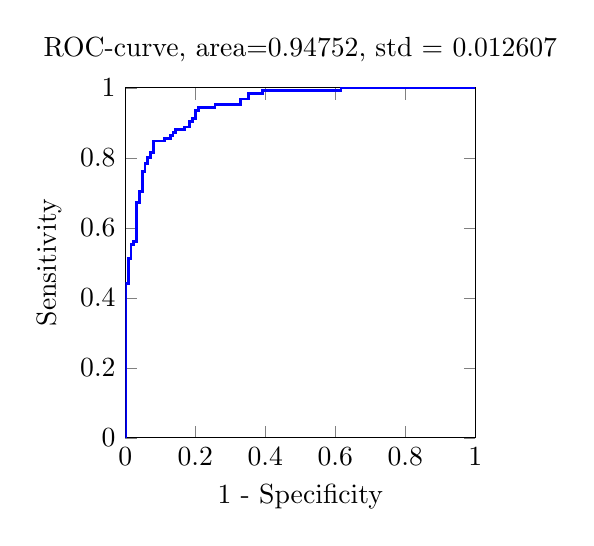
\begin{tikzpicture}

\begin{axis}[%
width=1.75in,
height=1.75in,
scale only axis,
xmin=0,
xmax=1,
xlabel={1 - Specificity},
ymin=0,
ymax=1,
ylabel={Sensitivity},
title={ROC-curve, area=0.94752, std = 0.012607}
]
\addplot [color=blue,solid,line width=1.0pt,forget plot]
  table[row sep=crcr]{%
0	0\\
0	0.008\\
0	0.016\\
0	0.024\\
0	0.032\\
0	0.04\\
0	0.048\\
0	0.056\\
0	0.064\\
0	0.072\\
0	0.08\\
0	0.088\\
0	0.096\\
0	0.104\\
0	0.112\\
0	0.12\\
0	0.128\\
0	0.136\\
0	0.144\\
0	0.152\\
0	0.16\\
0	0.168\\
0	0.176\\
0	0.184\\
0	0.192\\
0	0.2\\
0	0.208\\
0	0.216\\
0	0.224\\
0	0.232\\
0	0.24\\
0	0.248\\
0	0.256\\
0	0.264\\
0	0.272\\
0	0.28\\
0	0.288\\
0	0.296\\
0	0.304\\
0	0.312\\
0	0.32\\
0	0.328\\
0	0.336\\
0	0.344\\
0	0.352\\
0	0.36\\
0	0.368\\
0	0.376\\
0	0.384\\
0	0.392\\
0	0.4\\
0	0.408\\
0	0.416\\
0	0.424\\
0	0.432\\
0	0.44\\
0.008	0.44\\
0.008	0.448\\
0.008	0.456\\
0.008	0.464\\
0.008	0.472\\
0.008	0.48\\
0.008	0.488\\
0.008	0.496\\
0.008	0.504\\
0.008	0.512\\
0.016	0.512\\
0.016	0.52\\
0.016	0.528\\
0.016	0.536\\
0.016	0.544\\
0.016	0.552\\
0.024	0.552\\
0.024	0.56\\
0.032	0.56\\
0.032	0.568\\
0.032	0.576\\
0.032	0.584\\
0.032	0.592\\
0.032	0.6\\
0.032	0.608\\
0.032	0.616\\
0.032	0.624\\
0.032	0.632\\
0.032	0.64\\
0.032	0.648\\
0.032	0.656\\
0.032	0.664\\
0.032	0.672\\
0.04	0.672\\
0.04	0.68\\
0.04	0.688\\
0.04	0.696\\
0.04	0.704\\
0.048	0.704\\
0.048	0.712\\
0.048	0.72\\
0.048	0.728\\
0.048	0.736\\
0.048	0.744\\
0.048	0.752\\
0.048	0.76\\
0.056	0.76\\
0.056	0.768\\
0.056	0.776\\
0.056	0.784\\
0.064	0.784\\
0.064	0.792\\
0.064	0.8\\
0.072	0.8\\
0.072	0.808\\
0.072	0.816\\
0.08	0.816\\
0.08	0.824\\
0.08	0.832\\
0.08	0.84\\
0.08	0.848\\
0.088	0.848\\
0.096	0.848\\
0.104	0.848\\
0.112	0.848\\
0.112	0.856\\
0.12	0.856\\
0.128	0.856\\
0.128	0.864\\
0.136	0.864\\
0.136	0.872\\
0.144	0.872\\
0.144	0.88\\
0.152	0.88\\
0.16	0.88\\
0.168	0.88\\
0.168	0.888\\
0.176	0.888\\
0.184	0.888\\
0.184	0.896\\
0.184	0.904\\
0.192	0.904\\
0.192	0.912\\
0.2	0.912\\
0.2	0.92\\
0.2	0.928\\
0.2	0.936\\
0.208	0.936\\
0.208	0.944\\
0.216	0.944\\
0.224	0.944\\
0.232	0.944\\
0.24	0.944\\
0.248	0.944\\
0.256	0.944\\
0.256	0.952\\
0.264	0.952\\
0.272	0.952\\
0.28	0.952\\
0.288	0.952\\
0.296	0.952\\
0.304	0.952\\
0.312	0.952\\
0.32	0.952\\
0.328	0.952\\
0.328	0.96\\
0.328	0.968\\
0.336	0.968\\
0.344	0.968\\
0.352	0.968\\
0.352	0.976\\
0.352	0.984\\
0.36	0.984\\
0.368	0.984\\
0.376	0.984\\
0.384	0.984\\
0.392	0.984\\
0.392	0.992\\
0.4	0.992\\
0.408	0.992\\
0.416	0.992\\
0.424	0.992\\
0.432	0.992\\
0.44	0.992\\
0.448	0.992\\
0.456	0.992\\
0.464	0.992\\
0.472	0.992\\
0.48	0.992\\
0.488	0.992\\
0.496	0.992\\
0.504	0.992\\
0.512	0.992\\
0.52	0.992\\
0.528	0.992\\
0.536	0.992\\
0.544	0.992\\
0.552	0.992\\
0.56	0.992\\
0.568	0.992\\
0.576	0.992\\
0.584	0.992\\
0.592	0.992\\
0.6	0.992\\
0.608	0.992\\
0.616	0.992\\
0.616	1\\
0.624	1\\
0.632	1\\
0.64	1\\
0.648	1\\
0.656	1\\
0.664	1\\
0.672	1\\
0.68	1\\
0.688	1\\
0.696	1\\
0.704	1\\
0.712	1\\
0.72	1\\
0.728	1\\
0.736	1\\
0.744	1\\
0.752	1\\
0.76	1\\
0.768	1\\
0.776	1\\
0.784	1\\
0.792	1\\
0.8	1\\
0.808	1\\
0.816	1\\
0.824	1\\
0.832	1\\
0.84	1\\
0.848	1\\
0.856	1\\
0.864	1\\
0.872	1\\
0.88	1\\
0.888	1\\
0.896	1\\
0.904	1\\
0.912	1\\
0.92	1\\
0.928	1\\
0.936	1\\
0.944	1\\
0.952	1\\
0.96	1\\
0.968	1\\
0.976	1\\
0.984	1\\
0.992	1\\
1	1\\
};
\end{axis}
\end{tikzpicture}%
\end{document}
\caption{Radial basis function least squares support vector machines visualization and validation based roc curve.}
\label{fig:ripleyClass}
\end{figure}

\section{Breast Cancer Data-set}
The uci breast cancer set\footnote{\url{http://archive.ics.uci.edu/ml/datasets/Breast+Cancer+Wisconsin+\%28Diagnostic\%29}} contains 596 multidimensional-data points with tissue sample information such as smoothness, compactness, concavity, etc. The data is annotated, with labels indicating healthy or cancerous samples. 400 training and 169 validation measurements are included. Data points have more then 3 dimensions it is this not possible to visualize them using conventional methods. Therefore different classifiers will be trained and evaluated using their roc-curves. The roc-curves of automatically tuned linear and rbf-classifiers are shown in figure~\ref{fig:breastROC}. Both classifiers perform equally well, only around two to five percent of samples is missclassified using automatically tuned machines with either of the two kernels. 
\begin{figure}
\input{../src/tikz/breastLinRoc.tex}
% This file was created by matlab2tikz.
% Minimal pgfplots version: 1.3
%
%The latest updates can be retrieved from
%  http://www.mathworks.com/matlabcentral/fileexchange/22022-matlab2tikz
%where you can also make suggestions and rate matlab2tikz.
%
\documentclass[tikz]{standalone}
\usepackage{pgfplots}
\usepackage{grffile}
\pgfplotsset{compat=newest}
\usetikzlibrary{plotmarks}
\usepackage{amsmath}

\begin{document}
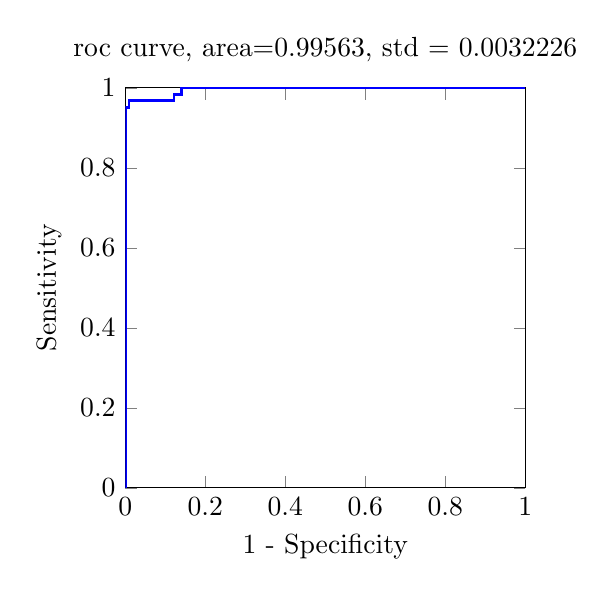
\begin{tikzpicture}

\begin{axis}[%
width=2.0in,
height=2.0in,
scale only axis,
xmin=0,
xmax=1,
xlabel={1 - Specificity},
ymin=0,
ymax=1,
ylabel={Sensitivity},
title={roc curve, area=0.99563, std = 0.0032226}
]
\addplot [color=blue,solid,line width=1.0pt,forget plot]
  table[row sep=crcr]{%
0	0\\
0	0.0161290322580645\\
0	0.032258064516129\\
0	0.0483870967741935\\
0	0.0645161290322581\\
0	0.0806451612903226\\
0	0.0967741935483871\\
0	0.112903225806452\\
0	0.129032258064516\\
0	0.145161290322581\\
0	0.161290322580645\\
0	0.17741935483871\\
0	0.193548387096774\\
0	0.209677419354839\\
0	0.225806451612903\\
0	0.241935483870968\\
0	0.258064516129032\\
0	0.274193548387097\\
0	0.290322580645161\\
0	0.306451612903226\\
0	0.32258064516129\\
0	0.338709677419355\\
0	0.354838709677419\\
0	0.370967741935484\\
0	0.387096774193548\\
0	0.403225806451613\\
0	0.419354838709677\\
0	0.435483870967742\\
0	0.451612903225806\\
0	0.467741935483871\\
0	0.483870967741935\\
0	0.5\\
0	0.516129032258065\\
0	0.532258064516129\\
0	0.548387096774194\\
0	0.564516129032258\\
0	0.580645161290323\\
0	0.596774193548387\\
0	0.612903225806452\\
0	0.629032258064516\\
0	0.645161290322581\\
0	0.661290322580645\\
0	0.67741935483871\\
0	0.693548387096774\\
0	0.709677419354839\\
0	0.725806451612903\\
0	0.741935483870968\\
0	0.758064516129032\\
0	0.774193548387097\\
0	0.790322580645161\\
0	0.806451612903226\\
0	0.82258064516129\\
0	0.838709677419355\\
0	0.854838709677419\\
0	0.870967741935484\\
0	0.887096774193548\\
0	0.903225806451613\\
0	0.919354838709677\\
0	0.935483870967742\\
0	0.951612903225806\\
0.00934579439252336	0.951612903225806\\
0.00934579439252336	0.967741935483871\\
0.0186915887850467	0.967741935483871\\
0.0280373831775701	0.967741935483871\\
0.0373831775700935	0.967741935483871\\
0.0467289719626168	0.967741935483871\\
0.0560747663551402	0.967741935483871\\
0.0654205607476635	0.967741935483871\\
0.0747663551401869	0.967741935483871\\
0.0841121495327103	0.967741935483871\\
0.0934579439252336	0.967741935483871\\
0.102803738317757	0.967741935483871\\
0.11214953271028	0.967741935483871\\
0.121495327102804	0.967741935483871\\
0.121495327102804	0.983870967741935\\
0.130841121495327	0.983870967741935\\
0.14018691588785	0.983870967741935\\
0.14018691588785	1\\
0.149532710280374	1\\
0.158878504672897	1\\
0.168224299065421	1\\
0.177570093457944	1\\
0.186915887850467	1\\
0.196261682242991	1\\
0.205607476635514	1\\
0.214953271028037	1\\
0.224299065420561	1\\
0.233644859813084	1\\
0.242990654205607	1\\
0.252336448598131	1\\
0.261682242990654	1\\
0.271028037383178	1\\
0.280373831775701	1\\
0.289719626168224	1\\
0.299065420560748	1\\
0.308411214953271	1\\
0.317757009345794	1\\
0.327102803738318	1\\
0.336448598130841	1\\
0.345794392523364	1\\
0.355140186915888	1\\
0.364485981308411	1\\
0.373831775700935	1\\
0.383177570093458	1\\
0.392523364485981	1\\
0.401869158878505	1\\
0.411214953271028	1\\
0.420560747663551	1\\
0.429906542056075	1\\
0.439252336448598	1\\
0.448598130841121	1\\
0.457943925233645	1\\
0.467289719626168	1\\
0.476635514018692	1\\
0.485981308411215	1\\
0.495327102803738	1\\
0.504672897196262	1\\
0.514018691588785	1\\
0.523364485981308	1\\
0.532710280373832	1\\
0.542056074766355	1\\
0.551401869158878	1\\
0.560747663551402	1\\
0.570093457943925	1\\
0.579439252336449	1\\
0.588785046728972	1\\
0.598130841121495	1\\
0.607476635514019	1\\
0.616822429906542	1\\
0.626168224299065	1\\
0.635514018691589	1\\
0.644859813084112	1\\
0.654205607476635	1\\
0.663551401869159	1\\
0.672897196261682	1\\
0.682242990654206	1\\
0.691588785046729	1\\
0.700934579439252	1\\
0.710280373831776	1\\
0.719626168224299	1\\
0.728971962616822	1\\
0.738317757009346	1\\
0.747663551401869	1\\
0.757009345794392	1\\
0.766355140186916	1\\
0.775700934579439	1\\
0.785046728971963	1\\
0.794392523364486	1\\
0.803738317757009	1\\
0.813084112149533	1\\
0.822429906542056	1\\
0.831775700934579	1\\
0.841121495327103	1\\
0.850467289719626	1\\
0.85981308411215	1\\
0.869158878504673	1\\
0.878504672897196	1\\
0.88785046728972	1\\
0.897196261682243	1\\
0.906542056074766	1\\
0.91588785046729	1\\
0.925233644859813	1\\
0.934579439252336	1\\
0.94392523364486	1\\
0.953271028037383	1\\
0.962616822429907	1\\
0.97196261682243	1\\
0.981308411214953	1\\
0.990654205607477	1\\
1	1\\
};
\end{axis}
\end{tikzpicture}%
\end{document}
\caption{Linear and radial basis function lssvm classifier roc-curves for the breast-cancer data set.}
\label{fig:breastROC}
\end{figure}

\section{Diabetes Database}
In this example data from a study of diabetes cases among female Pima indians \footnote{\url{http://archive.ics.uci.edu/ml/machine-learning-databases/pima-indians-diabetes/pima-indians-diabetes.names}} is used. The data set consists of 300 training data points and 168 validation samples. Each point consists of information such as the number of past pregnancies, body mass index, plasma glucose concentration and so on. 
Again for multi-dimensional data sets such as this one visualization is not trivial. Thus classifiers will once more be compared using their roc-curves. A linear and radial basis function svm has been trained. Their roc-plots are shown in figure~\ref{fig:diabetesROC}. 
\begin{figure}
% This file was created by matlab2tikz.
% Minimal pgfplots version: 1.3
%
%The latest updates can be retrieved from
%  http://www.mathworks.com/matlabcentral/fileexchange/22022-matlab2tikz
%where you can also make suggestions and rate matlab2tikz.
%
\documentclass[tikz]{standalone}
\usepackage{pgfplots}
\usepackage{grffile}
\pgfplotsset{compat=newest}
\usetikzlibrary{plotmarks}
\usepackage{amsmath}

\begin{document}
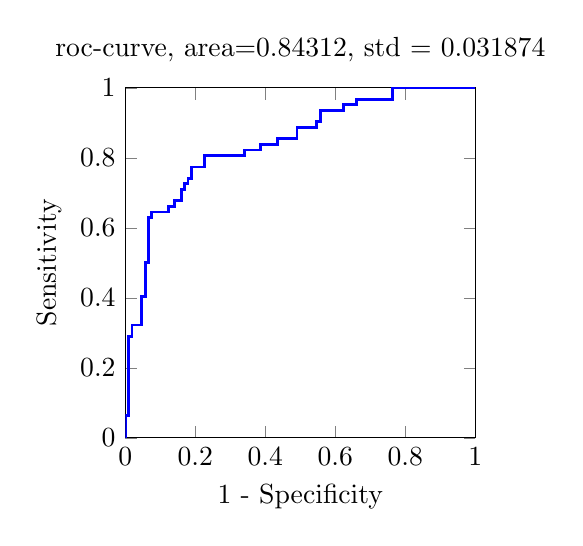
\begin{tikzpicture}

\begin{axis}[%
width=1.75in,
height=1.75in,
scale only axis,
xmin=0,
xmax=1,
xlabel={1 - Specificity},
ymin=0,
ymax=1,
ylabel={Sensitivity},
title={roc-curve, area=0.84312, std = 0.031874}
]
\addplot [color=blue,solid,line width=1.0pt,forget plot]
  table[row sep=crcr]{%
0	0\\
0	0.0161290322580645\\
0	0.032258064516129\\
0	0.0483870967741935\\
0	0.0645161290322581\\
0.00943396226415094	0.0645161290322581\\
0.00943396226415094	0.0806451612903226\\
0.00943396226415094	0.0967741935483871\\
0.00943396226415094	0.112903225806452\\
0.00943396226415094	0.129032258064516\\
0.00943396226415094	0.145161290322581\\
0.00943396226415094	0.161290322580645\\
0.00943396226415094	0.17741935483871\\
0.00943396226415094	0.193548387096774\\
0.00943396226415094	0.209677419354839\\
0.00943396226415094	0.225806451612903\\
0.00943396226415094	0.241935483870968\\
0.00943396226415094	0.258064516129032\\
0.00943396226415094	0.274193548387097\\
0.00943396226415094	0.290322580645161\\
0.0188679245283019	0.290322580645161\\
0.0188679245283019	0.306451612903226\\
0.0188679245283019	0.32258064516129\\
0.0283018867924528	0.32258064516129\\
0.0377358490566038	0.32258064516129\\
0.0471698113207547	0.32258064516129\\
0.0471698113207547	0.338709677419355\\
0.0471698113207547	0.354838709677419\\
0.0471698113207547	0.370967741935484\\
0.0471698113207547	0.387096774193548\\
0.0471698113207547	0.403225806451613\\
0.0566037735849057	0.403225806451613\\
0.0566037735849057	0.419354838709677\\
0.0566037735849057	0.435483870967742\\
0.0566037735849057	0.451612903225806\\
0.0566037735849057	0.467741935483871\\
0.0566037735849057	0.483870967741935\\
0.0566037735849057	0.5\\
0.0660377358490566	0.5\\
0.0660377358490566	0.516129032258065\\
0.0660377358490566	0.532258064516129\\
0.0660377358490566	0.548387096774194\\
0.0660377358490566	0.564516129032258\\
0.0660377358490566	0.580645161290323\\
0.0660377358490566	0.596774193548387\\
0.0660377358490566	0.612903225806452\\
0.0660377358490566	0.629032258064516\\
0.0754716981132075	0.629032258064516\\
0.0754716981132075	0.645161290322581\\
0.0849056603773585	0.645161290322581\\
0.0943396226415094	0.645161290322581\\
0.10377358490566	0.645161290322581\\
0.113207547169811	0.645161290322581\\
0.122641509433962	0.645161290322581\\
0.122641509433962	0.661290322580645\\
0.132075471698113	0.661290322580645\\
0.141509433962264	0.661290322580645\\
0.141509433962264	0.67741935483871\\
0.150943396226415	0.67741935483871\\
0.160377358490566	0.67741935483871\\
0.160377358490566	0.693548387096774\\
0.160377358490566	0.709677419354839\\
0.169811320754717	0.709677419354839\\
0.169811320754717	0.725806451612903\\
0.179245283018868	0.725806451612903\\
0.179245283018868	0.741935483870968\\
0.188679245283019	0.741935483870968\\
0.188679245283019	0.758064516129032\\
0.188679245283019	0.774193548387097\\
0.19811320754717	0.774193548387097\\
0.207547169811321	0.774193548387097\\
0.216981132075472	0.774193548387097\\
0.226415094339623	0.774193548387097\\
0.226415094339623	0.790322580645161\\
0.226415094339623	0.806451612903226\\
0.235849056603774	0.806451612903226\\
0.245283018867925	0.806451612903226\\
0.254716981132075	0.806451612903226\\
0.264150943396226	0.806451612903226\\
0.273584905660377	0.806451612903226\\
0.283018867924528	0.806451612903226\\
0.292452830188679	0.806451612903226\\
0.30188679245283	0.806451612903226\\
0.311320754716981	0.806451612903226\\
0.320754716981132	0.806451612903226\\
0.330188679245283	0.806451612903226\\
0.339622641509434	0.806451612903226\\
0.339622641509434	0.82258064516129\\
0.349056603773585	0.82258064516129\\
0.358490566037736	0.82258064516129\\
0.367924528301887	0.82258064516129\\
0.377358490566038	0.82258064516129\\
0.386792452830189	0.82258064516129\\
0.386792452830189	0.838709677419355\\
0.39622641509434	0.838709677419355\\
0.405660377358491	0.838709677419355\\
0.415094339622642	0.838709677419355\\
0.424528301886792	0.838709677419355\\
0.433962264150943	0.838709677419355\\
0.433962264150943	0.854838709677419\\
0.443396226415094	0.854838709677419\\
0.452830188679245	0.854838709677419\\
0.462264150943396	0.854838709677419\\
0.471698113207547	0.854838709677419\\
0.481132075471698	0.854838709677419\\
0.490566037735849	0.854838709677419\\
0.490566037735849	0.870967741935484\\
0.490566037735849	0.887096774193548\\
0.5	0.887096774193548\\
0.509433962264151	0.887096774193548\\
0.518867924528302	0.887096774193548\\
0.528301886792453	0.887096774193548\\
0.537735849056604	0.887096774193548\\
0.547169811320755	0.887096774193548\\
0.547169811320755	0.903225806451613\\
0.556603773584906	0.903225806451613\\
0.556603773584906	0.919354838709677\\
0.556603773584906	0.935483870967742\\
0.566037735849057	0.935483870967742\\
0.575471698113208	0.935483870967742\\
0.584905660377358	0.935483870967742\\
0.594339622641509	0.935483870967742\\
0.60377358490566	0.935483870967742\\
0.613207547169811	0.935483870967742\\
0.622641509433962	0.935483870967742\\
0.622641509433962	0.951612903225806\\
0.632075471698113	0.951612903225806\\
0.641509433962264	0.951612903225806\\
0.650943396226415	0.951612903225806\\
0.660377358490566	0.951612903225806\\
0.660377358490566	0.967741935483871\\
0.669811320754717	0.967741935483871\\
0.679245283018868	0.967741935483871\\
0.688679245283019	0.967741935483871\\
0.69811320754717	0.967741935483871\\
0.707547169811321	0.967741935483871\\
0.716981132075472	0.967741935483871\\
0.726415094339623	0.967741935483871\\
0.735849056603774	0.967741935483871\\
0.745283018867924	0.967741935483871\\
0.754716981132076	0.967741935483871\\
0.764150943396226	0.967741935483871\\
0.764150943396226	0.983870967741935\\
0.764150943396226	1\\
0.773584905660377	1\\
0.783018867924528	1\\
0.792452830188679	1\\
0.80188679245283	1\\
0.811320754716981	1\\
0.820754716981132	1\\
0.830188679245283	1\\
0.839622641509434	1\\
0.849056603773585	1\\
0.858490566037736	1\\
0.867924528301887	1\\
0.877358490566038	1\\
0.886792452830189	1\\
0.89622641509434	1\\
0.905660377358491	1\\
0.915094339622642	1\\
0.924528301886792	1\\
0.933962264150943	1\\
0.943396226415094	1\\
0.952830188679245	1\\
0.962264150943396	1\\
0.971698113207547	1\\
0.981132075471698	1\\
0.990566037735849	1\\
1	1\\
};
\end{axis}
\end{tikzpicture}%
\end{document}
% This file was created by matlab2tikz.
% Minimal pgfplots version: 1.3
%
%The latest updates can be retrieved from
%  http://www.mathworks.com/matlabcentral/fileexchange/22022-matlab2tikz
%where you can also make suggestions and rate matlab2tikz.
%
\documentclass[tikz]{standalone}
\usepackage{pgfplots}
\usepackage{grffile}
\pgfplotsset{compat=newest}
\usetikzlibrary{plotmarks}
\usepackage{amsmath}

\begin{document}
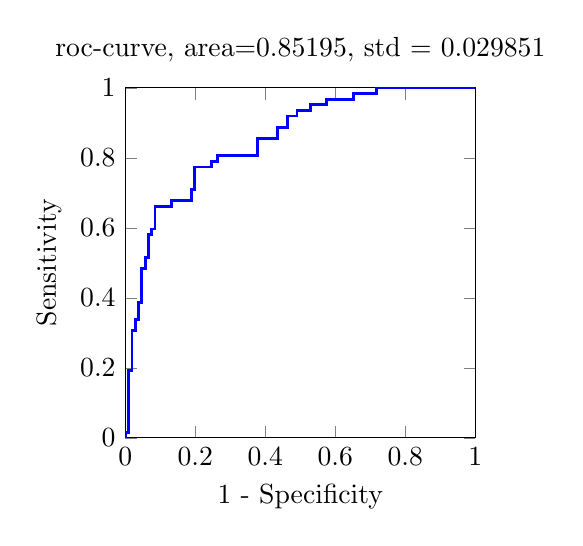
\begin{tikzpicture}

\begin{axis}[%
width=1.75in,
height=1.75in,
scale only axis,
xmin=0,
xmax=1,
xlabel={1 - Specificity},
ymin=0,
ymax=1,
ylabel={Sensitivity},
title={roc-curve, area=0.85195, std = 0.029851}
]
\addplot [color=blue,solid,line width=1.0pt,forget plot]
  table[row sep=crcr]{%
0	0\\
0	0.0161290322580645\\
0.00943396226415094	0.0161290322580645\\
0.00943396226415094	0.032258064516129\\
0.00943396226415094	0.0483870967741935\\
0.00943396226415094	0.0645161290322581\\
0.00943396226415094	0.0806451612903226\\
0.00943396226415094	0.0967741935483871\\
0.00943396226415094	0.112903225806452\\
0.00943396226415094	0.129032258064516\\
0.00943396226415094	0.145161290322581\\
0.00943396226415094	0.161290322580645\\
0.00943396226415094	0.17741935483871\\
0.00943396226415094	0.193548387096774\\
0.0188679245283019	0.193548387096774\\
0.0188679245283019	0.209677419354839\\
0.0188679245283019	0.225806451612903\\
0.0188679245283019	0.241935483870968\\
0.0188679245283019	0.258064516129032\\
0.0188679245283019	0.274193548387097\\
0.0188679245283019	0.290322580645161\\
0.0188679245283019	0.306451612903226\\
0.0283018867924528	0.306451612903226\\
0.0283018867924528	0.32258064516129\\
0.0283018867924528	0.338709677419355\\
0.0377358490566038	0.338709677419355\\
0.0377358490566038	0.354838709677419\\
0.0377358490566038	0.370967741935484\\
0.0377358490566038	0.387096774193548\\
0.0471698113207547	0.387096774193548\\
0.0471698113207547	0.403225806451613\\
0.0471698113207547	0.419354838709677\\
0.0471698113207547	0.435483870967742\\
0.0471698113207547	0.451612903225806\\
0.0471698113207547	0.467741935483871\\
0.0471698113207547	0.483870967741935\\
0.0566037735849057	0.483870967741935\\
0.0566037735849057	0.5\\
0.0566037735849057	0.516129032258065\\
0.0660377358490566	0.516129032258065\\
0.0660377358490566	0.532258064516129\\
0.0660377358490566	0.548387096774194\\
0.0660377358490566	0.564516129032258\\
0.0660377358490566	0.580645161290323\\
0.0754716981132075	0.580645161290323\\
0.0754716981132075	0.596774193548387\\
0.0849056603773585	0.596774193548387\\
0.0849056603773585	0.612903225806452\\
0.0849056603773585	0.629032258064516\\
0.0849056603773585	0.645161290322581\\
0.0849056603773585	0.661290322580645\\
0.0943396226415094	0.661290322580645\\
0.10377358490566	0.661290322580645\\
0.113207547169811	0.661290322580645\\
0.122641509433962	0.661290322580645\\
0.132075471698113	0.661290322580645\\
0.132075471698113	0.67741935483871\\
0.141509433962264	0.67741935483871\\
0.150943396226415	0.67741935483871\\
0.160377358490566	0.67741935483871\\
0.169811320754717	0.67741935483871\\
0.179245283018868	0.67741935483871\\
0.188679245283019	0.67741935483871\\
0.188679245283019	0.693548387096774\\
0.188679245283019	0.709677419354839\\
0.19811320754717	0.709677419354839\\
0.19811320754717	0.725806451612903\\
0.19811320754717	0.741935483870968\\
0.19811320754717	0.758064516129032\\
0.19811320754717	0.774193548387097\\
0.207547169811321	0.774193548387097\\
0.216981132075472	0.774193548387097\\
0.226415094339623	0.774193548387097\\
0.235849056603774	0.774193548387097\\
0.245283018867925	0.774193548387097\\
0.245283018867925	0.790322580645161\\
0.254716981132075	0.790322580645161\\
0.264150943396226	0.790322580645161\\
0.264150943396226	0.806451612903226\\
0.273584905660377	0.806451612903226\\
0.283018867924528	0.806451612903226\\
0.292452830188679	0.806451612903226\\
0.30188679245283	0.806451612903226\\
0.311320754716981	0.806451612903226\\
0.320754716981132	0.806451612903226\\
0.330188679245283	0.806451612903226\\
0.339622641509434	0.806451612903226\\
0.349056603773585	0.806451612903226\\
0.358490566037736	0.806451612903226\\
0.367924528301887	0.806451612903226\\
0.377358490566038	0.806451612903226\\
0.377358490566038	0.82258064516129\\
0.377358490566038	0.838709677419355\\
0.377358490566038	0.854838709677419\\
0.386792452830189	0.854838709677419\\
0.39622641509434	0.854838709677419\\
0.405660377358491	0.854838709677419\\
0.415094339622642	0.854838709677419\\
0.424528301886792	0.854838709677419\\
0.433962264150943	0.854838709677419\\
0.433962264150943	0.870967741935484\\
0.433962264150943	0.887096774193548\\
0.443396226415094	0.887096774193548\\
0.452830188679245	0.887096774193548\\
0.462264150943396	0.887096774193548\\
0.462264150943396	0.903225806451613\\
0.462264150943396	0.919354838709677\\
0.471698113207547	0.919354838709677\\
0.481132075471698	0.919354838709677\\
0.490566037735849	0.919354838709677\\
0.490566037735849	0.935483870967742\\
0.5	0.935483870967742\\
0.509433962264151	0.935483870967742\\
0.518867924528302	0.935483870967742\\
0.528301886792453	0.935483870967742\\
0.528301886792453	0.951612903225806\\
0.537735849056604	0.951612903225806\\
0.547169811320755	0.951612903225806\\
0.556603773584906	0.951612903225806\\
0.566037735849057	0.951612903225806\\
0.575471698113208	0.951612903225806\\
0.575471698113208	0.967741935483871\\
0.584905660377358	0.967741935483871\\
0.594339622641509	0.967741935483871\\
0.60377358490566	0.967741935483871\\
0.613207547169811	0.967741935483871\\
0.622641509433962	0.967741935483871\\
0.632075471698113	0.967741935483871\\
0.641509433962264	0.967741935483871\\
0.650943396226415	0.967741935483871\\
0.650943396226415	0.983870967741935\\
0.660377358490566	0.983870967741935\\
0.669811320754717	0.983870967741935\\
0.679245283018868	0.983870967741935\\
0.688679245283019	0.983870967741935\\
0.69811320754717	0.983870967741935\\
0.707547169811321	0.983870967741935\\
0.716981132075472	0.983870967741935\\
0.716981132075472	1\\
0.726415094339623	1\\
0.735849056603774	1\\
0.745283018867924	1\\
0.754716981132076	1\\
0.764150943396226	1\\
0.773584905660377	1\\
0.783018867924528	1\\
0.792452830188679	1\\
0.80188679245283	1\\
0.811320754716981	1\\
0.820754716981132	1\\
0.830188679245283	1\\
0.839622641509434	1\\
0.849056603773585	1\\
0.858490566037736	1\\
0.867924528301887	1\\
0.877358490566038	1\\
0.886792452830189	1\\
0.89622641509434	1\\
0.905660377358491	1\\
0.915094339622642	1\\
0.924528301886792	1\\
0.933962264150943	1\\
0.943396226415094	1\\
0.952830188679245	1\\
0.962264150943396	1\\
0.971698113207547	1\\
0.981132075471698	1\\
0.990566037735849	1\\
1	1\\
};
\end{axis}
\end{tikzpicture}%
\end{document}
\caption{Linear and radial basis function lssvm classifier roc-curves for the diabetes data set.}
\label{fig:diabetesROC}
\end{figure}
Again the two classifiers perform similarly with the linear classifier being correct in 74\% of cases and the radial basis function delivering correct classification in  77.8\% of all validation cases.  
